% vocabulary diversity
% segmentation on sentences
% document variables and meta-data
% relationship of document units to summary statistics
% seriality (not available from matrix)
% implement dfmSort
% FIX REGEX in CODE

%\documentclass[11pt]{beamer}
\documentclass[11pt,handout]{beamer}

\usepackage[all]{xy}
\usepackage{hyperref}
\usepackage{setspace}

\title[Day 2:\newline Descriptive Statistics]{Day 2: Descriptive statistical methods for textual analysis}
\author[]{Pablo Barber\'{a} \& Kenneth Benoit}\institute[LSE
2016]{MY 459: Quantitative Text Analysis}

\date{January 15, 2018}

\begin{document}

\begin{frame}%<handout:0>
 \titlepage
\end{frame}


\begin{frame}
 \frametitle{Day 2 Outline}
 \begin{itemize}
  \item Problems to watch out for
  \item Getting to know your texts
  \item Key words in context
  \item Revisiting feature selection
  \item Stemming v. lemmatization
  \item Feature weighting strategies
  \item Collocations
  \item Named entity recognition
  \item Brief preview of Lab assignment
 \end{itemize}
\end{frame}

\begin{frame}
 \frametitle{Problems you are likely to encounter}
 \begin{itemize}
  \item \pause Problems with encoding
  \item \pause Problems file formats
  \item \pause Extraneous junk (page footers, numbers, titles, etc)
  \item \pause misspelllings
  \item \pause different normalizations (e.g. for Japanese)
 \end{itemize}
\end{frame}


\begin{frame}
  \frametitle{Simple descriptive table about texts: Describe your data!}
\scriptsize
  \centering
  \begin{tabular}{llrr}
\hline
Speaker		&	Party	&	Tokens	&
Types	\\
\hline\hline
Brian	Cowen	&	FF	&	 5,842 	&	 1,466 	\\
Brian	Lenihan	&	FF	&	 7,737 	&	 1,644 	\\
Ciaran	Cuffe	&	Green	&	 1,141 	&	 421 	\\
John	Gormley	(Edited) &	Green	&	 919 	&	 361 	\\
John	Gormley (Full)	&	Green	&	 2,998 	&	 868 	\\
Eamon	Ryan	&	Green	&	 1,513 	&	 481 	\\
Richard	Bruton	&	FG	&	 4,043 	&	 947 	\\
Enda	Kenny	&	FG	&	 3,863 	&	 1,055 	\\
Kieran	ODonnell	&	FG	&	 2,054 	&	 609 	\\
Joan	Burton	&	LAB	&	 5,728 	&	 1,471 	\\
Eamon	Gilmore	&	LAB	&	 3,780 	&	 1,082 	\\
Michael	Higgins	&	LAB	&	 1,139 	&	 437 	\\
Ruairi	Quinn	&	LAB	&	 1,182 	&	 413 	\\
Arthur	Morgan	&	SF	&	 6,448 	&	 1,452 	\\
Caoimhghin	O'Caolain	&	SF	&	 3,629 	&
1,035 	\\[1ex]
All Texts & & 49,019 & 4,840 \\[1ex]
\multicolumn{2}{l}{\emph{Min}}	&	 919 	&	 361 	\\
\multicolumn{2}{l}{\emph{Max}}	&	 7,737 	&	 1,644 	\\
\multicolumn{2}{l}{\emph{Median}}	&	 3,704 	&	 991 \\
\multicolumn{2}{l}{\em Hapaxes with Gormley Edited} & 67                 \\
\multicolumn{2}{l}{\em Hapaxes with Gormley Full Speech} & 69                 \\
\hline
  \end{tabular}

\end{frame}

\begin{frame}
 \frametitle{Exploring Texts: Key Words in Context}
 \begin{description}
  \pause \item[KWIC] \emph{Key words in context} Refers to the most
  common format for concordance lines.  A KWIC index is formed by
  sorting and aligning the words within an article title to allow each
  word (except the stop words) in titles to be searchable
  alphabetically in the index.
 \end{description}
 \begin{center}
  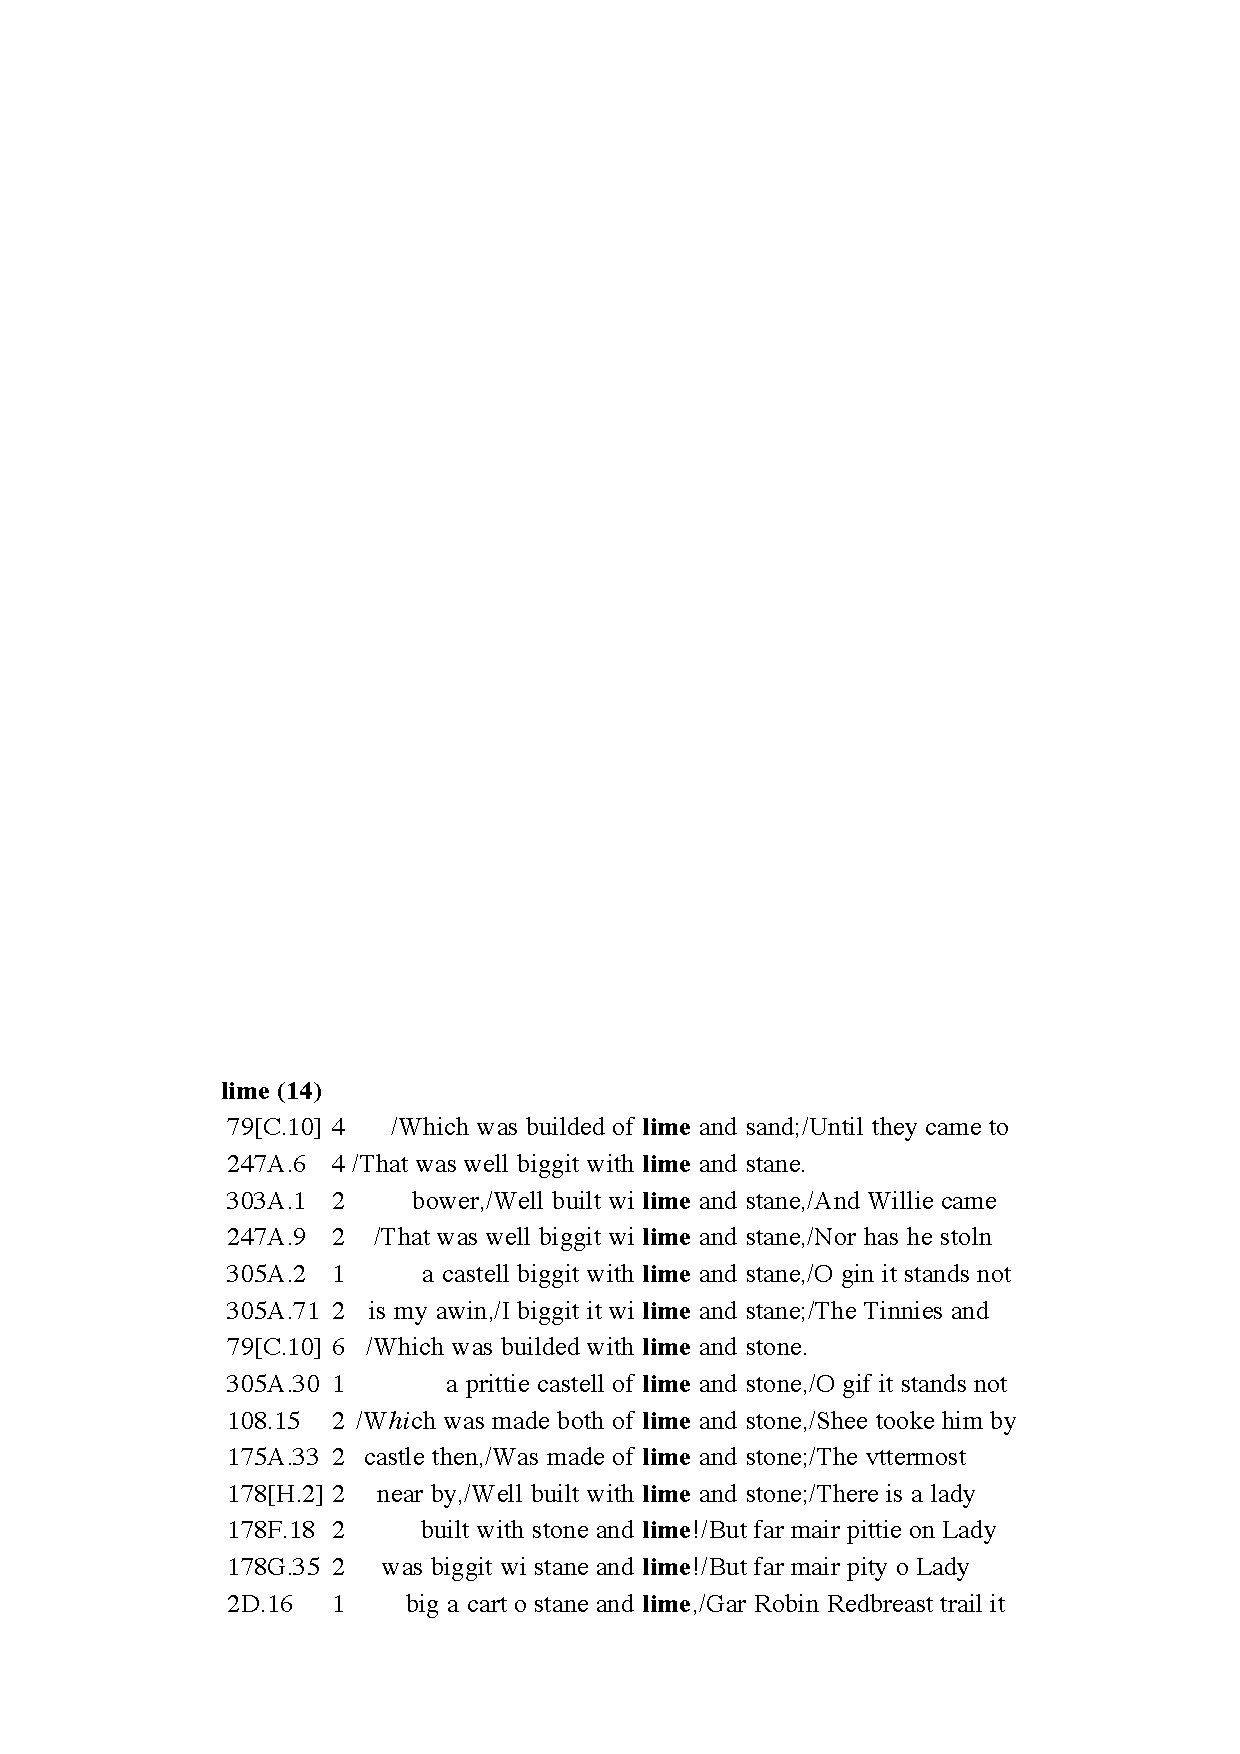
\includegraphics[width=7cm]{kwic.pdf}
 \end{center}
\end{frame}



\begin{frame}
 \frametitle{Another KWIC Example (Seale et al (2006)}
 \begin{center}
  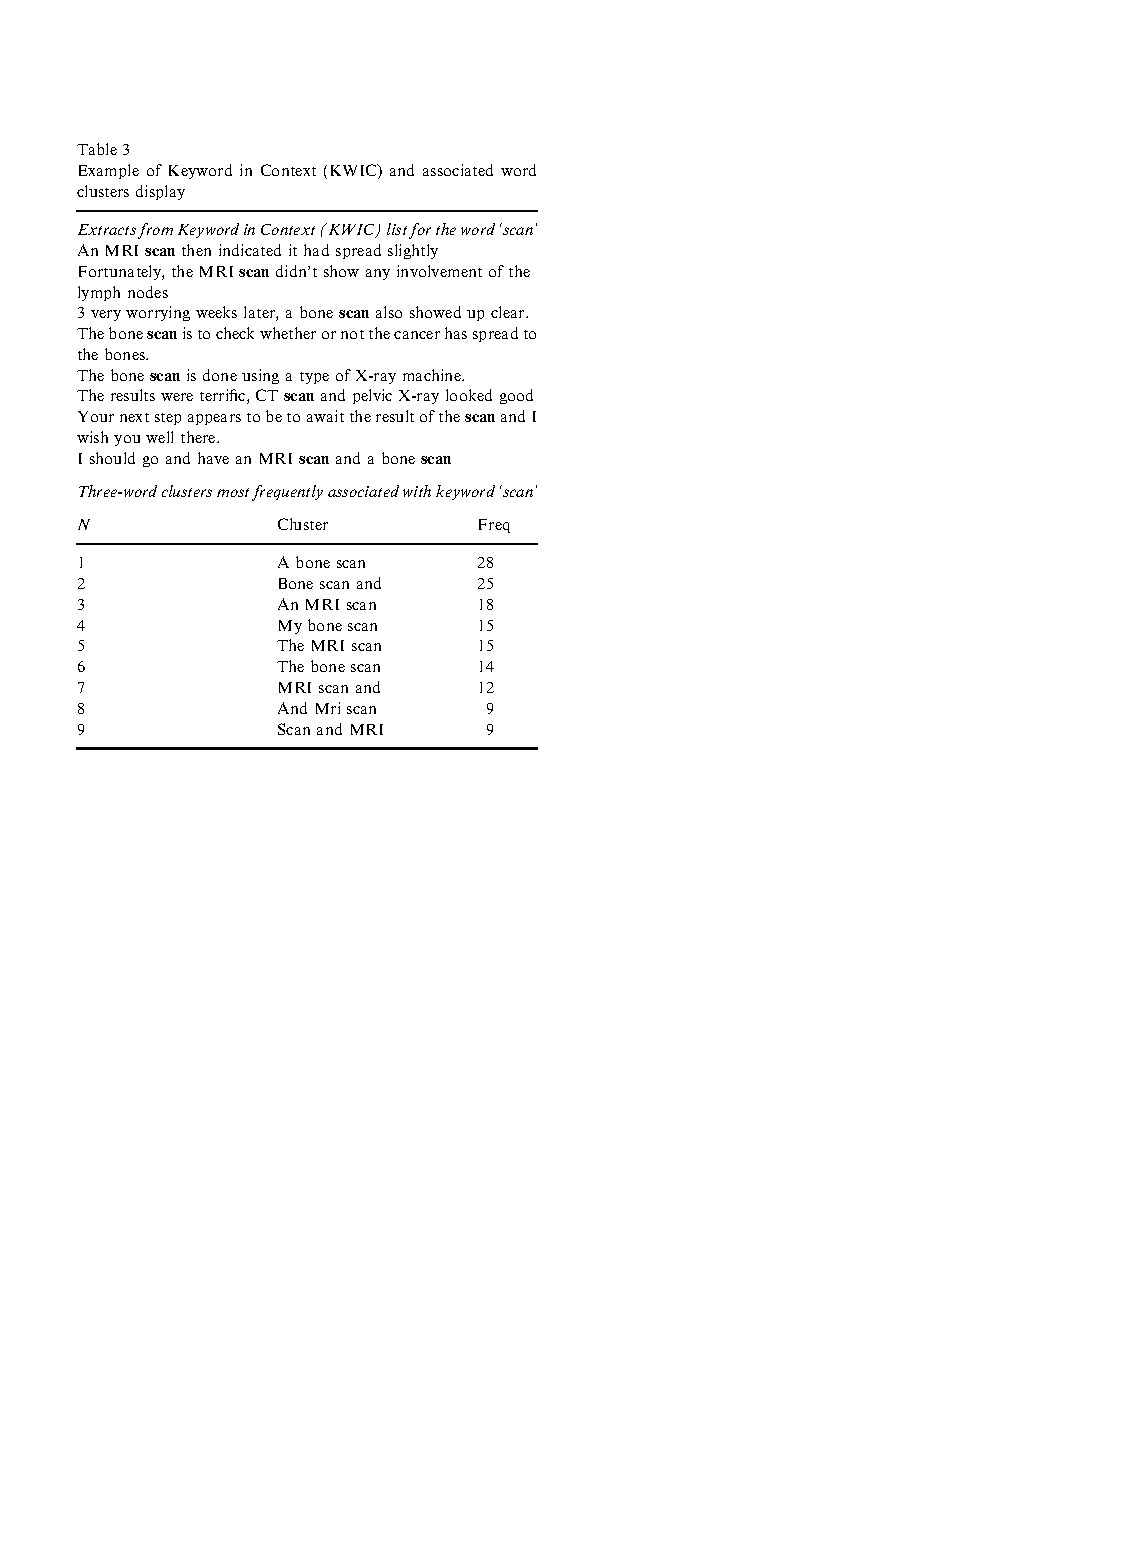
\includegraphics[width=6cm]{SealeKWIC.pdf}
 \end{center}
\end{frame}

\begin{frame}
 \frametitle{Another KWIC Example: Irish Budget Speeches}
 \begin{center}
  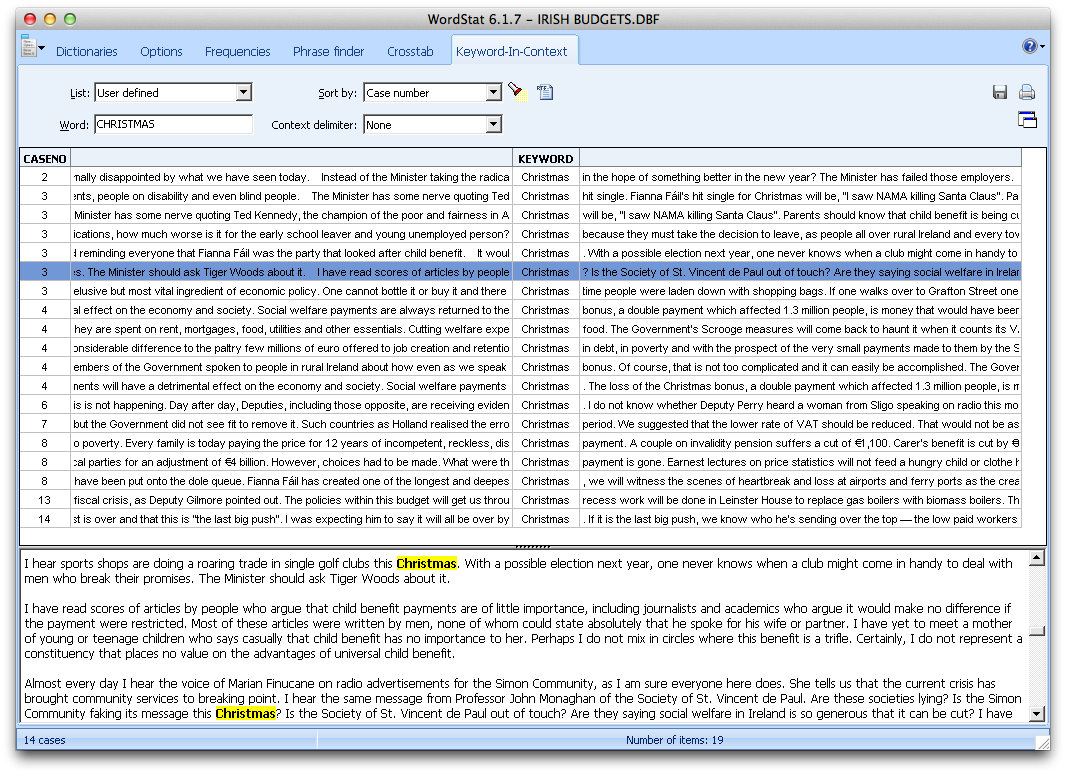
\includegraphics[width=10.5cm]{KWICWordstat.png}
 \end{center}
\end{frame}

\begin{frame}
 \frametitle{Irish Budget Speeches KIWC in \texttt{quanteda}}
 \begin{center}
  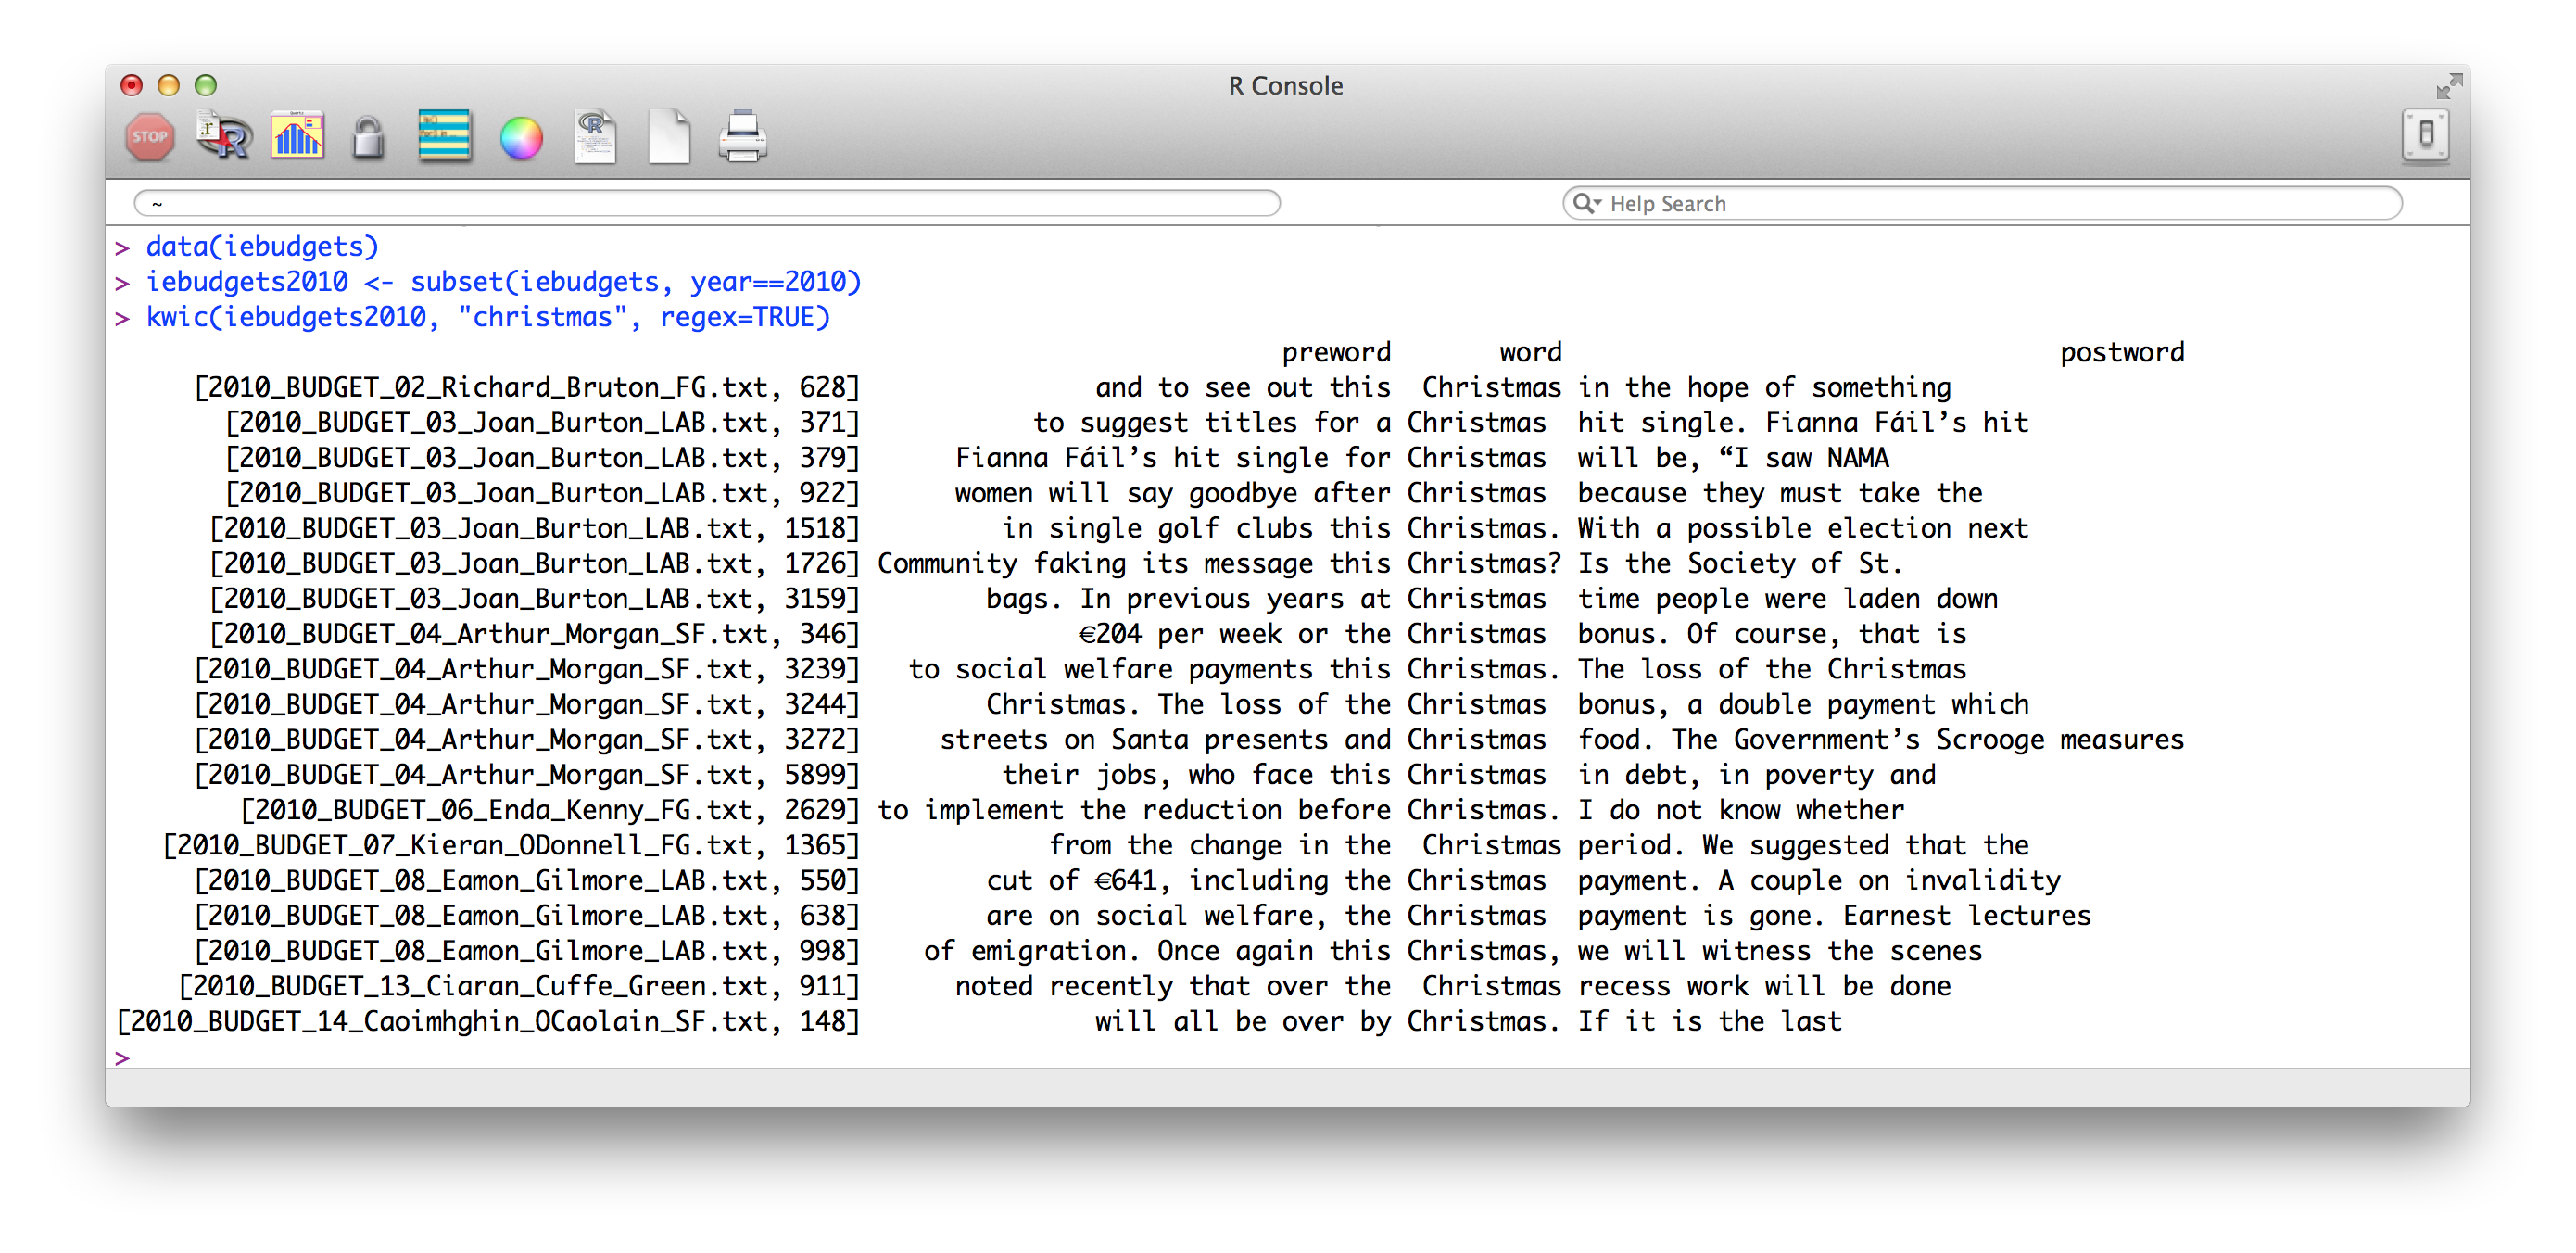
\includegraphics[width=1.1\textwidth]{KWICquanteda.png}
 \end{center}
\end{frame}


\begin{frame}
 \frametitle{Defining Features}
 \begin{itemize}
  \item words
  \item \pause word stems or lemmas: this is a form of defining \emph{equivalence classes} for word features
  \item \pause word segments, especially for languages using compound words,
        such as German, e.g. \newline
        \pause
        \htmladdnormallink{\emph{Rindfleischetikettierungsüberwachungsaufgabenübertragungsgesetz}}{http://www.telegraph.co.uk/news/worldnews/europe/germany/10095976/Germany-drops-its-longest-word-Rindfleischeti....html}
        \newline
        \pause {\footnotesize (the law concerning the delegation of duties for the supervision of cattle marking and the labelling of beef)} \newline
        \pause \emph{Saunauntensitzer}
 \end{itemize}
\end{frame}

\begin{frame}
 \frametitle{Defining Features (cont.)}
 \begin{itemize}
  \item ``word'' sequences, especially when inter-word delimiters
        (usually white space) are not commonly used, as in Chinese
        
\includegraphics{chinese.pdf}
  \item linguistic features, such as parts of speech
  \item (if qualitative coding is used) coded or annotated text
        segments
  \item linguistic features: parts of speech
 \end{itemize}
\end{frame}

\begin{frame}
  \frametitle{Stemming words}
  \begin{description}[<+->]
  \item[Lemmatization] refers to the algorithmic process of
    converting words to their lemma forms.  \pause
  \item[stemming] the
    process for reducing inflected (or sometimes derived) words to
    their stem, base or root form.  Different from
    \emph{lemmatization} in that stemmers operate on single words
    without knowledge of the context.
   \item[both] convert the morphological variants into stem or root terms
  \item[example:]
    \alert{\texttt{produc}} from \newline
    \texttt{production, producer, produce, produces, produced}
  \item[Why?] Reduce feature space by collapsing different words into a stem (e.g. ``happier'' and ``happily'' convey same meaning as ``happy'')
  \end{description}
\end{frame}

\begin{frame}
  \frametitle{Varieties of stemming algorithms}
  \begin{center}
    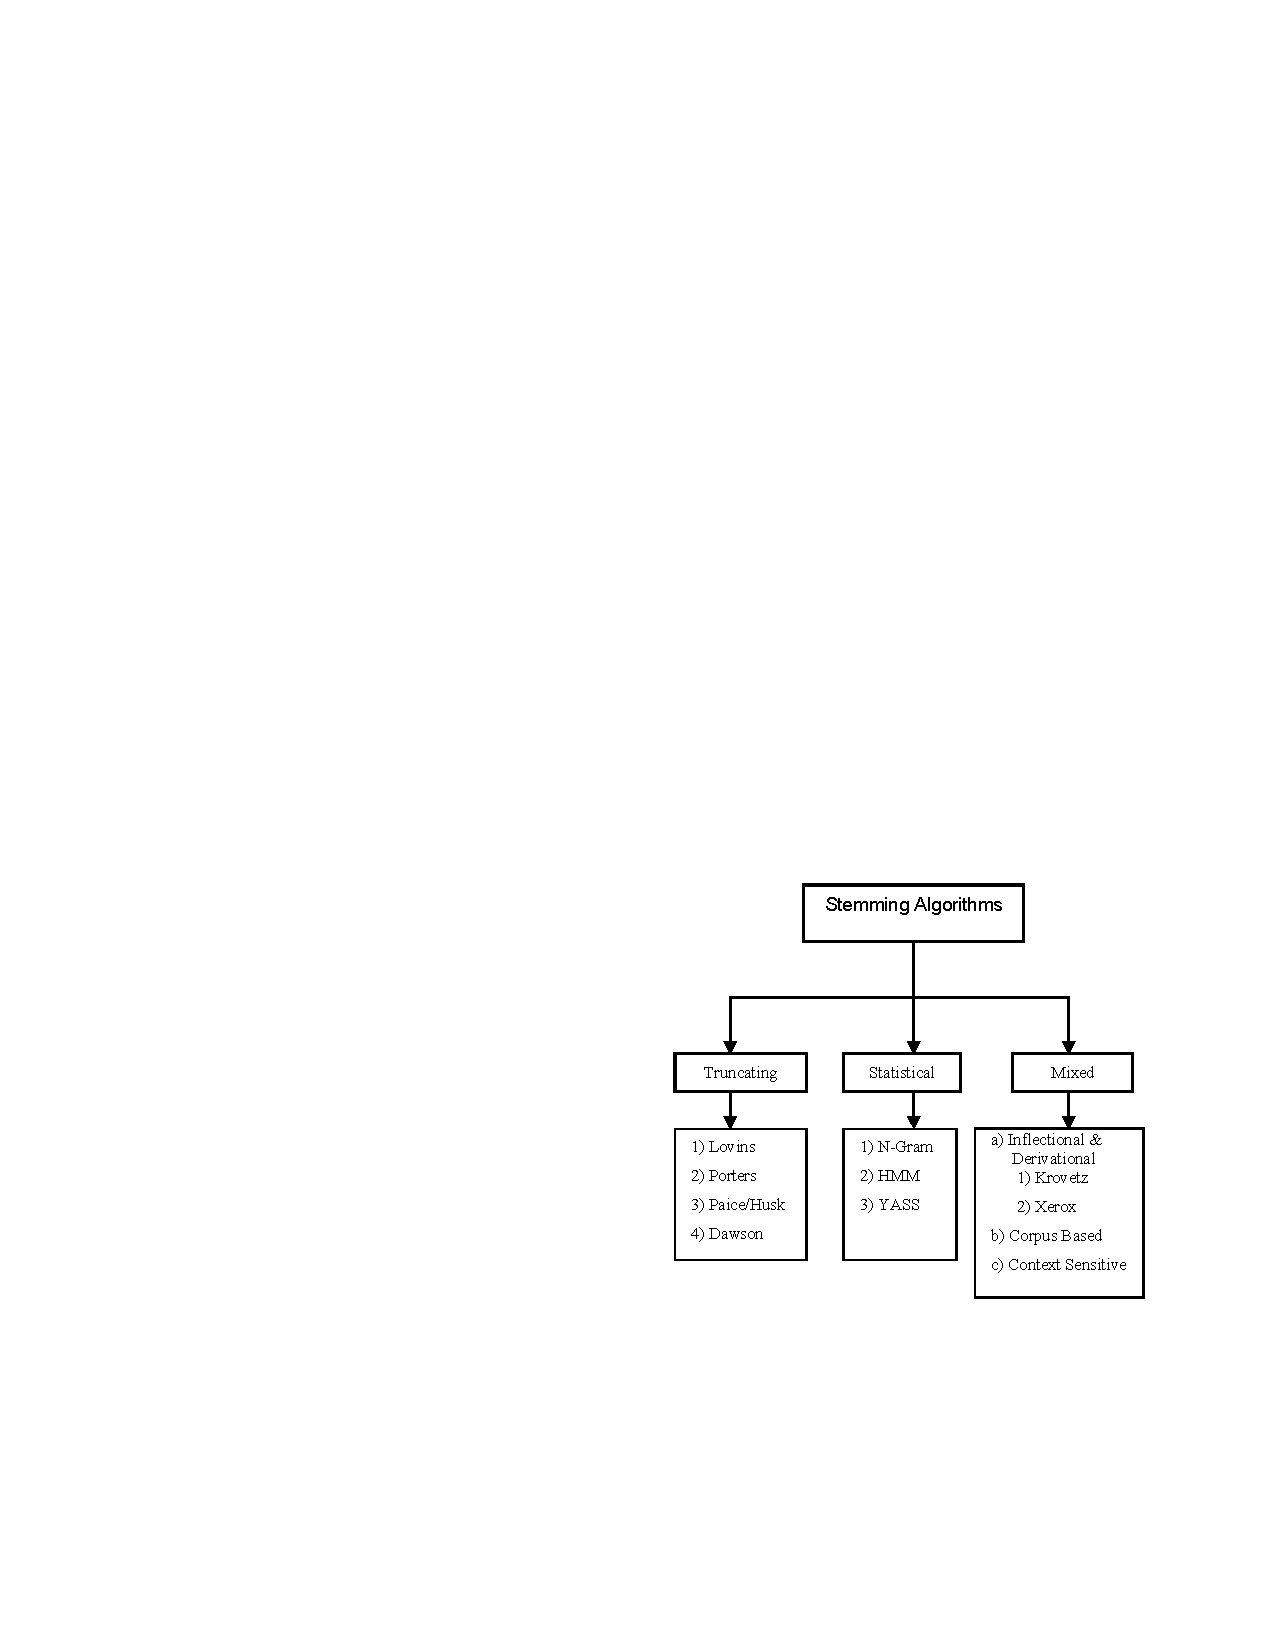
\includegraphics{stemming_algorithms.pdf}
  \end{center}
\end{frame}

\begin{frame}
  \frametitle{Issues with stemming approaches}
  \begin{itemize}[<+->]
  \item The most common is probably the \alert{Porter} stemmer
  \item But this set of rules gets many stems wrong, e.g.
    \begin{itemize}
    \item \texttt{policy} and \texttt{police} considered (wrongly) equivalent
    \item \texttt{general} becomes \texttt{gener}, \texttt{iteration}
      becomes \texttt{iter}
    \end{itemize}
  \item Other corpus-based, statistical, and mixed approaches designed
    to overcome these limitations
  \item Key for you is to be careful through inspection of
    morphological variants and their stemmed versions
  \item Sometimes not appropriate! e.g. Schofield and Minmo (2016) find that \small{``stemmers produce no meaningful improvement in likelihood and coherence (of topic models) and in fact can degrade topic stability''}
\end{itemize}
\end{frame}


\begin{frame}[fragile]
 \frametitle{Parts of speech}
 \begin{itemize}
  \item \htmladdnormallink{the Penn
              ``Treebank''}{https://www.ling.upenn.edu/courses/Fall_2003/ling001/penn_treebank_pos.html}
        is the standard scheme for tagging POS
        \vspace{.25cm}

        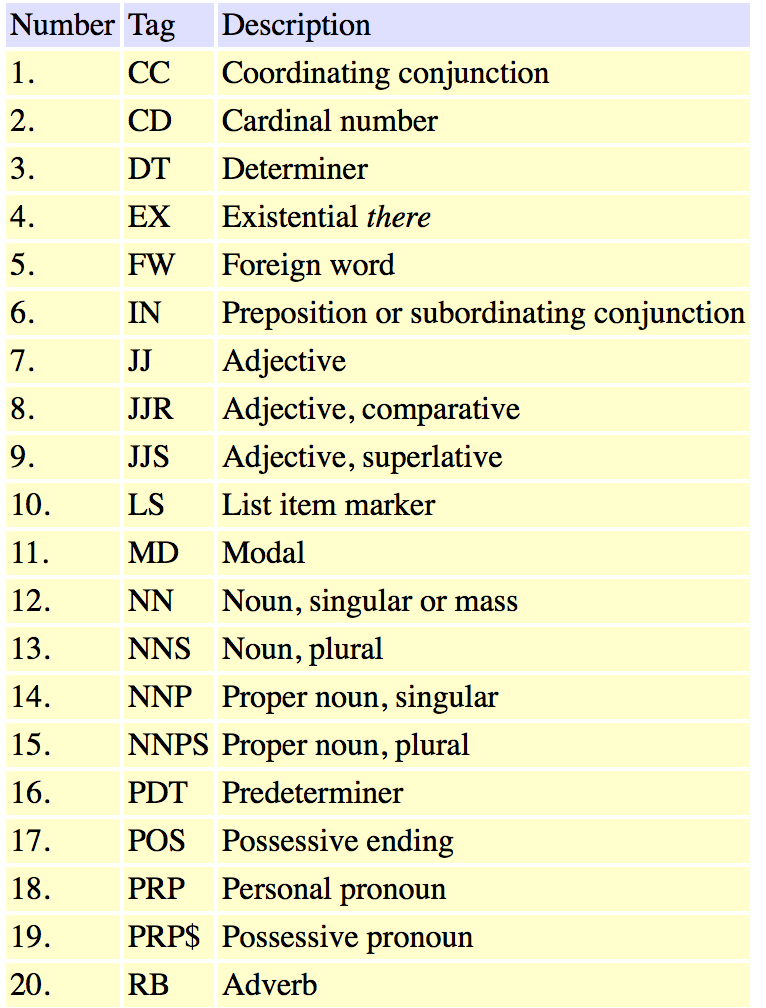
\includegraphics[width=5cm]{penntreebank1.png} 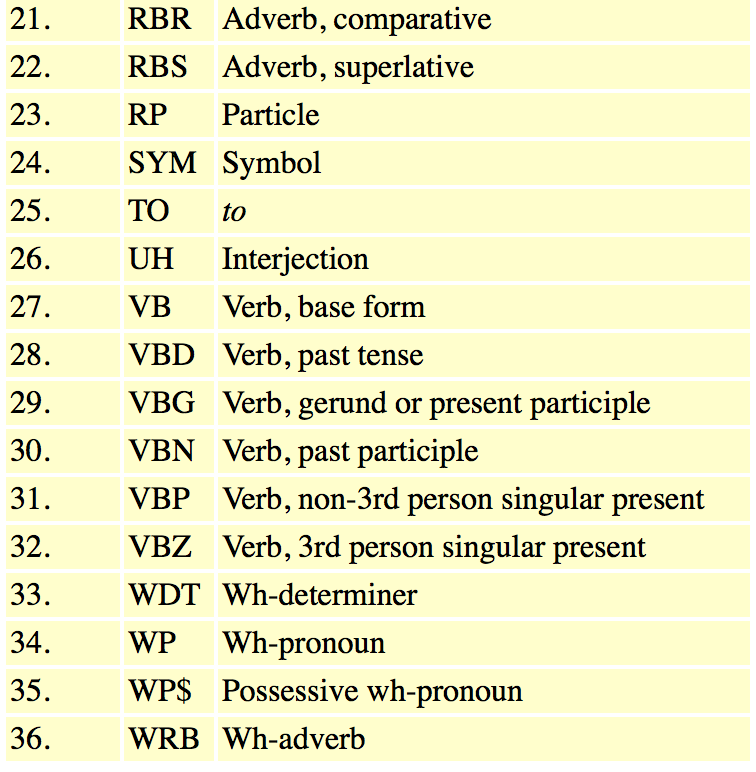
\includegraphics[width=5cm]{penntreebank2.png}
 \end{itemize}
\end{frame}

\begin{frame}[fragile]
 \frametitle{Parts of speech (cont.)}
 \scriptsize
 \begin{verbatim}
   > library("spacyr")
   > txt <- "Pierre Vinken, 61 years old, will join the board as a nonexecutive
             director Nov. 29.  Mr. Vinken is chairman of Elsevier N.V.,
             the Dutch publishing group."
   > spacy_parse(txt)
   doc_id sentence_id token_id        token        lemma   pos        entity
   1   text1           1        1       Pierre       pierre PROPN      PERSON_B
   2   text1           1        2       Vinken       vinken PROPN      PERSON_I
   3   text1           1        3            ,            , PUNCT
   4   text1           1        4           61           61   NUM        DATE_B
   5   text1           1        5        years         year  NOUN        DATE_I
   6   text1           1        6          old          old   ADJ        DATE_I
   7   text1           1        7            ,            , PUNCT
   8   text1           1        8         will         will  VERB
   9   text1           1        9         join         join  VERB
   10  text1           1       10          the          the   DET
   11  text1           1       11        board        board  NOUN
   12  text1           1       12           as           as   ADP
   13  text1           1       13            a            a   DET
   14  text1           1       14 nonexecutive nonexecutive   ADJ
   15  text1           1       15   \n           \n         SPACE
   16  text1           1       16     director     director  NOUN
   17  text1           1       17         Nov.         nov. PROPN        DATE_B
   18  text1           1       18           29           29   NUM        DATE_I
   19  text1           1       19            .            . PUNCT
 \end{verbatim}
\end{frame}

\begin{frame}[fragile]
 \frametitle{Parts of speech (cont.)}
 \scriptsize
 \begin{verbatim}
   20  text1           1       20                           SPACE
   21  text1           2        1          Mr.          mr. PROPN
   22  text1           2        2       Vinken       vinken PROPN      PERSON_B
   23  text1           2        3           is           be  VERB
   24  text1           2        4     chairman     chairman  NOUN
   25  text1           2        5           of           of   ADP
   26  text1           2        6     Elsevier     elsevier PROPN         ORG_B
   27  text1           2        7         N.V.         n.v. PROPN         ORG_I
   28  text1           2        8            ,            , PUNCT
   29  text1           2        9   \n           \n         SPACE WORK_OF_ART_B
   30  text1           2       10          the          the   DET WORK_OF_ART_I
   31  text1           2       11        Dutch        dutch   ADJ        NORP_B
   32  text1           2       12   publishing   publishing  NOUN
   33  text1           2       13        group        group  NOUN
   34  text1           2       14            .            . PUNCT
 \end{verbatim}
\end{frame}

\begin{frame}[fragile]
 \frametitle{Stemming v. lemmas}
 \scriptsize
 \begin{verbatim}
> library("quanteda")
> tokens(txt) %>% tokens_wordstem()
tokens from 1 document.
text1 :
[1] "Pierr"     "Vinken"    ","         "61"        "year"      "old"       ","         "will"
[9] "join"      "the"       "board"     "as"        "a"         "nonexecut" "director"  "Nov"
[17] "."         "29"        "."         "Mr"        "."         "Vinken"    "is"        "chairman"
[25] "of"        "Elsevier"  "N.V"       "."         ","         "the"       "Dutch"     "publish"
[33] "group"     "."

sp$lemma
[1] "pierre"       "vinken"       ","            "61"           "year"         "old"
[7] ","            "will"         "join"         "the"          "board"        "as"
[13] "a"            "nonexecutive" "\n        "   "director"     "nov."         "29"
[19] "."            " "            "mr."          "vinken"       "be"           "chairman"
[25] "of"           "elsevier"     "n.v."         ","            "\n        "   "the"
[31] "dutch"        "publishing"   "group"        "."
\end{verbatim}
\end{frame}




\begin{frame}
 \frametitle{Weighting strategies for feature counting}
 \begin{description}
  \item[term frequency] Some approaches trim very low-frequency words.
  Rationale: get rid of rare words that expand the feature matrix
  but matter little to substantive analysis
  \item[document frequency] Could eliminate words appearing in few documents
  \item[inverse document frequency] Conversely, could weight words
  more that appear in the most documents
  \item[\emph{tf-idf}] a combination of term frequency and inverse
  document frequency, common method for feature weighting
 \end{description}
\end{frame}

\begin{frame}
 \frametitle{Strategies for feature \emph{weighting}: tf-idf}
 \begin{itemize}
  \setlength{\itemsep}{3ex}
  \item $tf_{i,j} = \frac{n_{i,j}}{\sum_kn_{k,j}}$
        where $n_{i,j}$ is number of occurences of term $t_i$ in document
        $d_j$, $k$ is total number of terms in document $d_j$
  \item $idf_i = \mathrm{ln} \frac{|D|}{|\left\{ d_j: t_i \in d_j \right\} |}$

        where
        \begin{itemize}
         \item $|D|$ is the total number of documents in the set
         \item $|\left\{ d_j: t_i \in d_j \right\} |$ is the number of
               documents where the term $t_i$ appears (i.e. $n_{i,j}\neq 0$)
        \end{itemize}

  \item \emph{tf-idf}$_i = \mathit{tf}_{i,j} \cdot \mathit{idf}_i$
 \end{itemize}
\end{frame}

\begin{frame}
 \frametitle{Computation of tf-idf: Example}
 Example: We have 100 political party manifestos, each with 1000
 words.  The first document contains 16 instances of the word
 ``environment''; 40 of the manifestos contain the word
 ``environment''.
 \vspace{2ex}
 \begin{itemize}
  \setlength{\itemsep}{1.2ex}
  \item The \emph{term frequency} is $16/1000 = 0.016$
  \item The \emph{document frequency} is $100/40 = 2.5$, or
        ln$(2.5)=0.916$
  \item The \emph{tf-idf} will then be $0.016 * 0.916 = 0.0147$
  \item \pause If the word had only appeared in 15 of the 100 manifestos,
        then the \emph{tf-idf} would be 0.0304 (three times higher).
  \item \pause A high weight in tf-idf is reached by a high term frequency
        (in the given document) and a low document frequency of the term
        in the whole collection of documents; hence the \alert{weights hence tend to
        filter out common terms}
 \end{itemize}
\end{frame}



\begin{frame}
 \frametitle{Other weighting schemes}
 \begin{itemize}
  \item the SMART weighting scheme (Salton 1991, Salton et
        al):\newline
        \begin{small}The first letter in each triplet specifies the term frequency
         component of the weighting, the second the document frequency
         component, and the third the form of normalization used (not
         shown).  Example: \emph{lnn} means log-weighted term frequency, no idf, no
         normalization
        \end{small}
        \begin{center}
         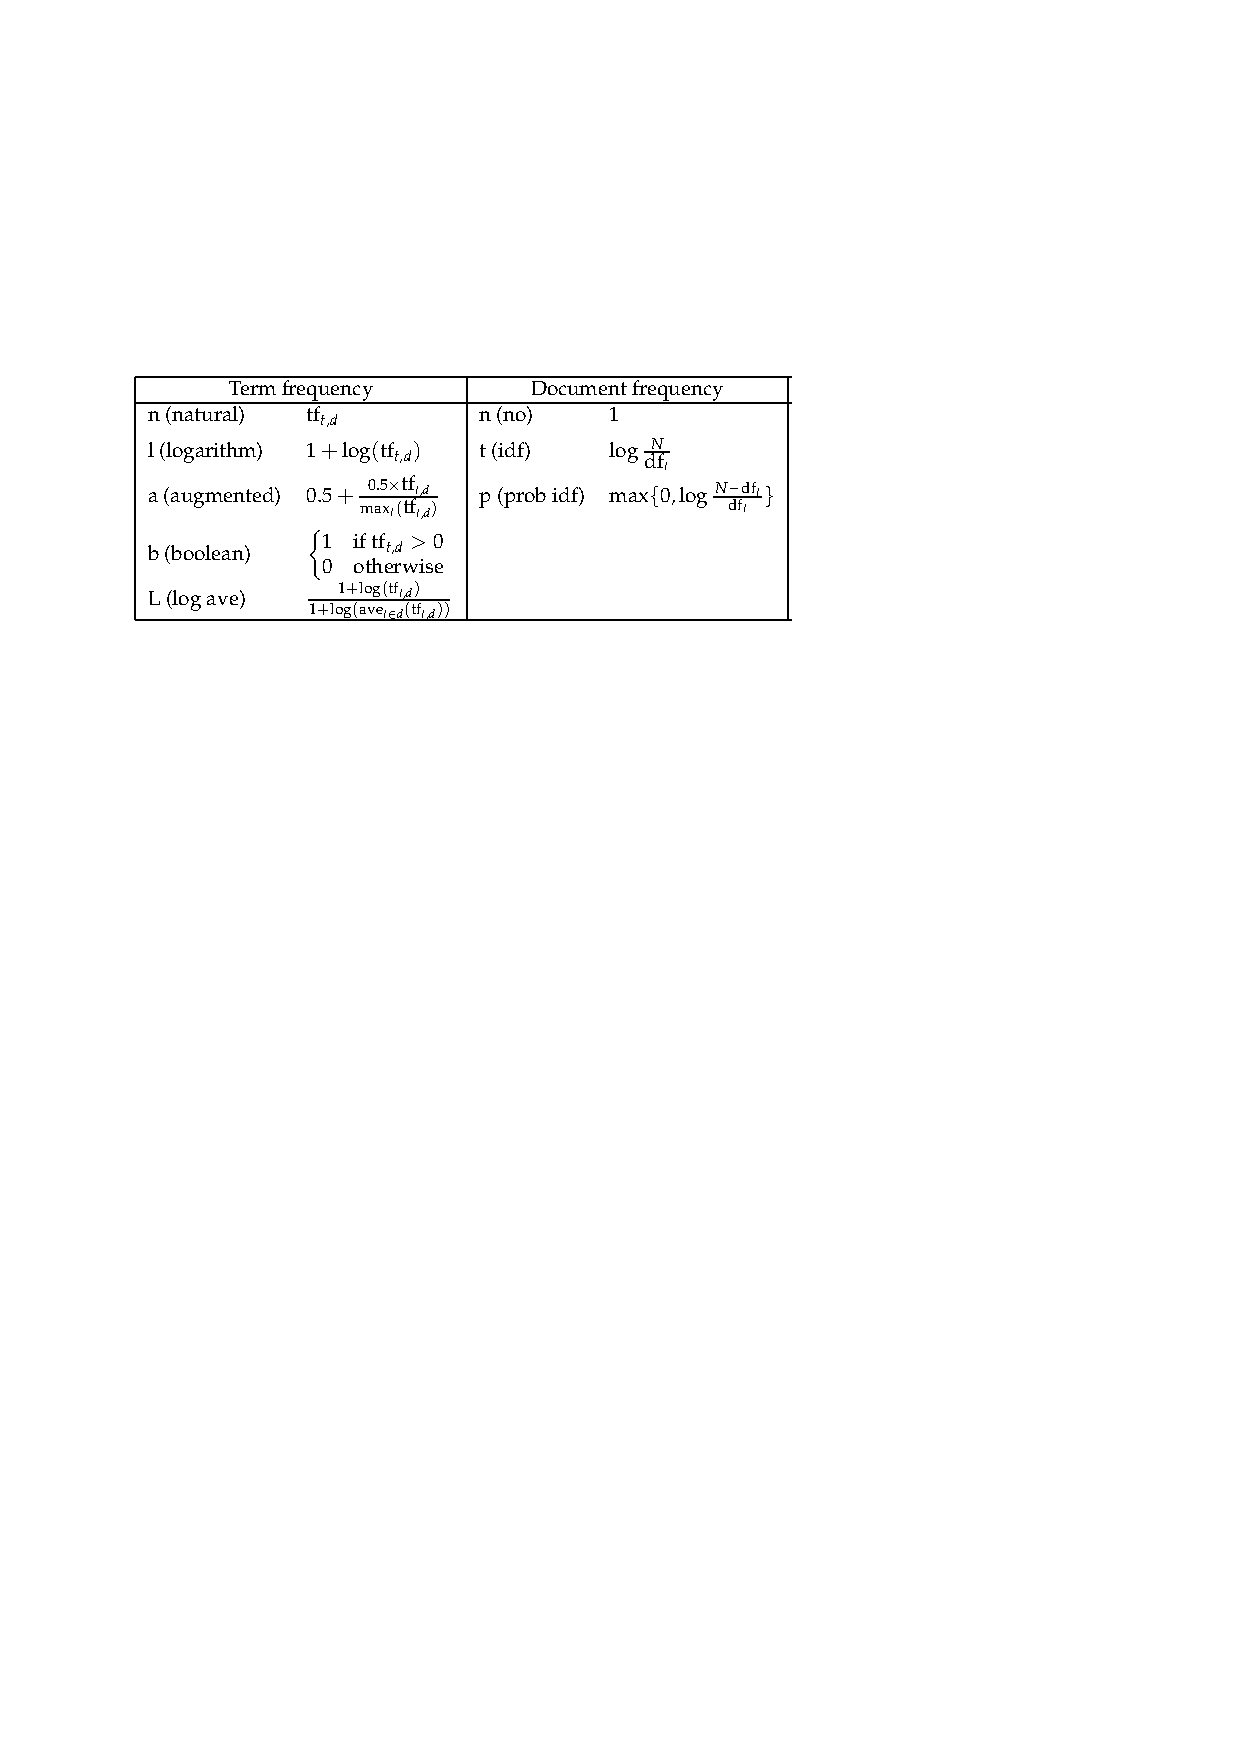
\includegraphics[width=10cm]{SMARTweightingscheme.pdf}
        \end{center}
  \item Note: Mostly used in information retrieval, although some use in
        machine learning
 \end{itemize}
\end{frame}




\begin{frame}
 \frametitle{Selecting more than words: collocations}
 \begin{description}
  \item[collocations] \alert{bigrams}, or \alert{trigrams}
  e.g. \emph{capital gains tax}
  \item[how to detect:] pairs occuring more than by chance, by measures
  of $\chi^2$ or \emph{mutual information} measures
  %  \begin{center}
  %  \end{center}
  \item[example:]
 \end{description}
 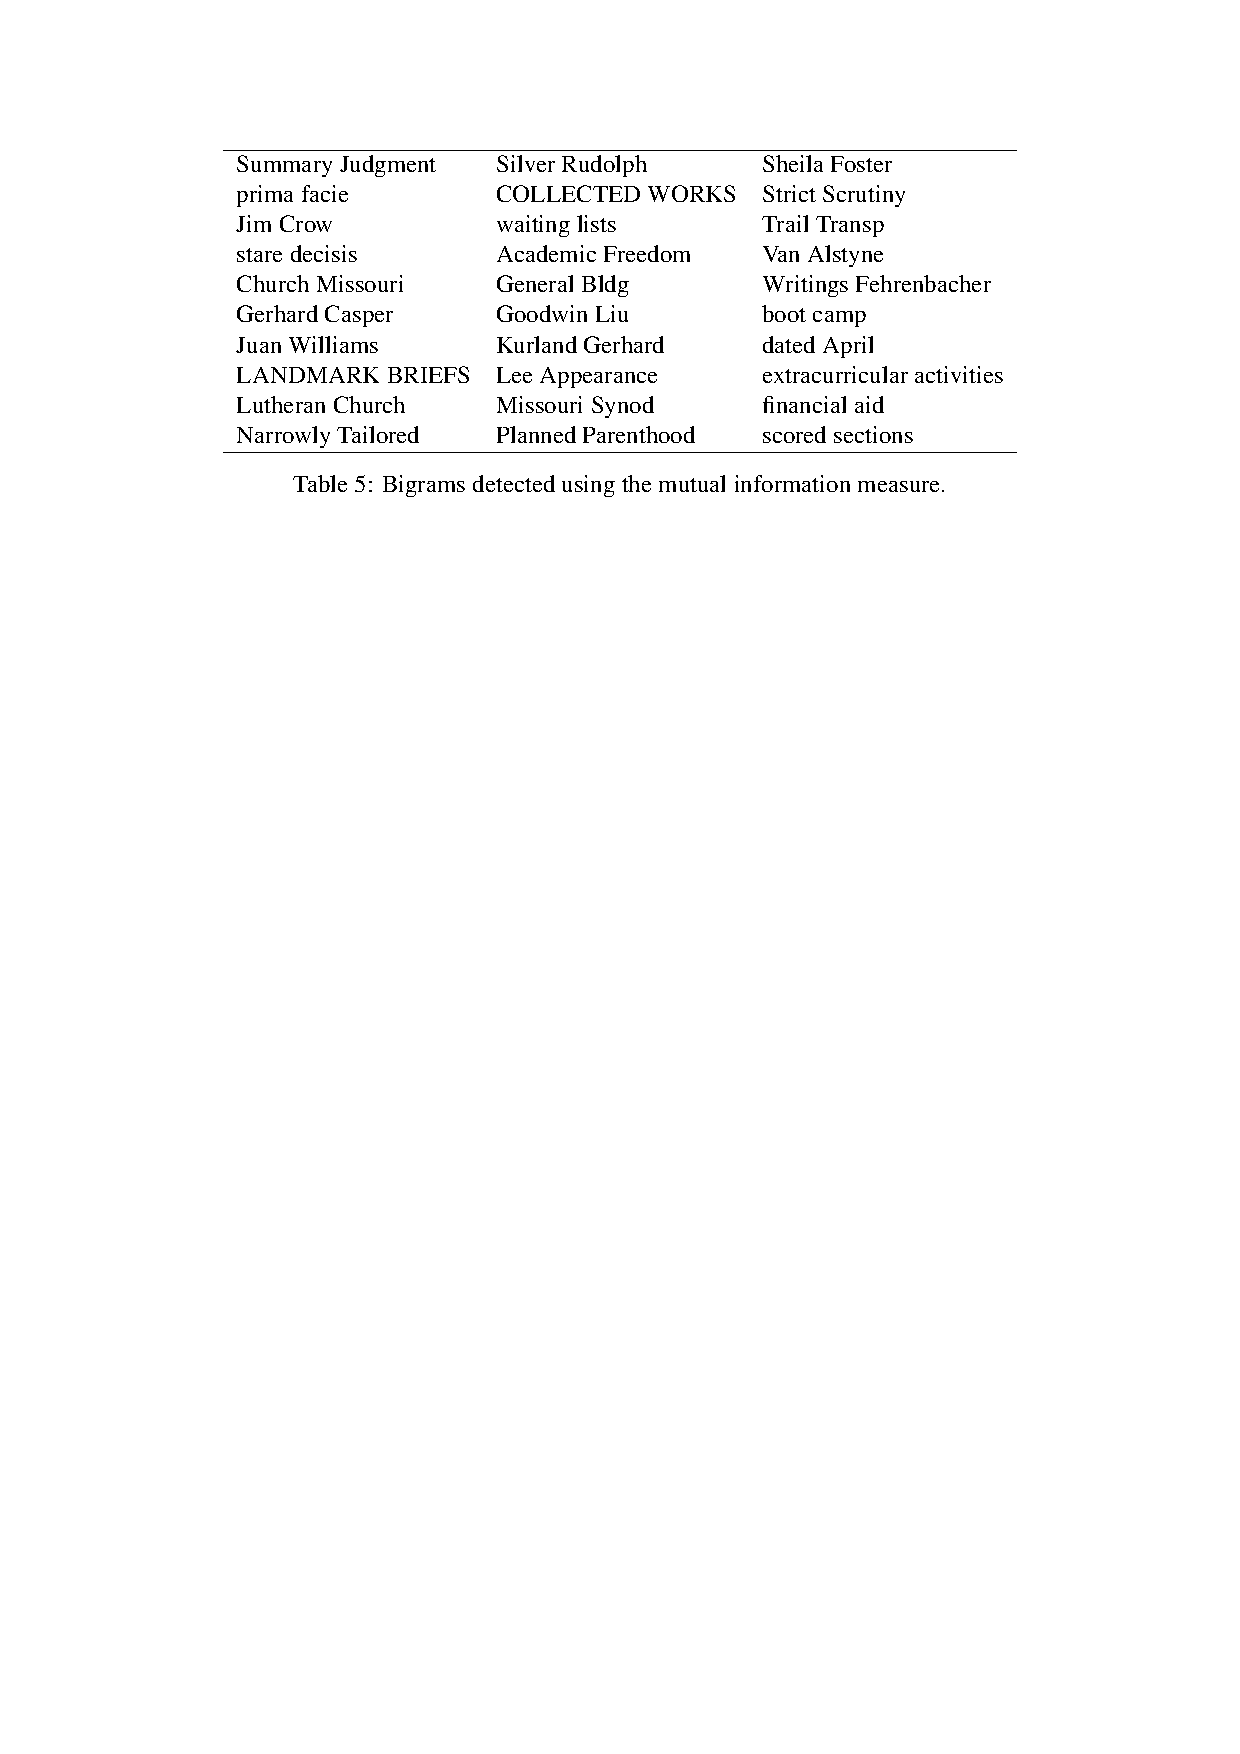
\includegraphics[width=10cm]{bigrams_amicus.pdf}
\end{frame}





\begin{frame}
 \frametitle{Identifying collocations}
 \begin{itemize}
  \item Does a given word occur next to another given word with a
        higher relative frequency than other words?
  \item If so, then it is a candidate for a collocation or ``word bigram''
  \item We can detect these using $\chi^2$ or likelihood ratio
        measures (Dunning paper)
  \item Implemented in quanteda as \texttt{collocations()}
 \end{itemize}
\end{frame}





\begin{frame}
 \frametitle{Getting texts into \texttt{quanteda}}
 \begin{itemize}
  \item text format issue
        \begin{itemize}
         \item text files
         \item zipped text files
         \item spreadsheets/CSV
         \item (pdfs)
         \item (Twitter feed)
        \end{itemize}
  \item encoding issue
  \item metadata and document variable management
 \end{itemize}
\end{frame}


\begin{frame}
 \frametitle{Identifying collocations}
 \begin{itemize}
  \item Does a given word occur next to another given word with a
        higher relative frequency than other words?
  \item If so, then it is a candidate for a collocation
  \item We can detect these using measures of association, such as a
        likelihood ratio, to detect word pairs that occur with greater
        than chance frequency, compared to an independence model
  \item The key is to distinguish ``true collocations'' from
        uninteresting word pairs/triplets/etc, such as ``of the''
  \item Implemented in quanteda as \texttt{collocations}
 \end{itemize}
\end{frame}

\begin{frame}
 \frametitle{Example}
 \begin{center}
  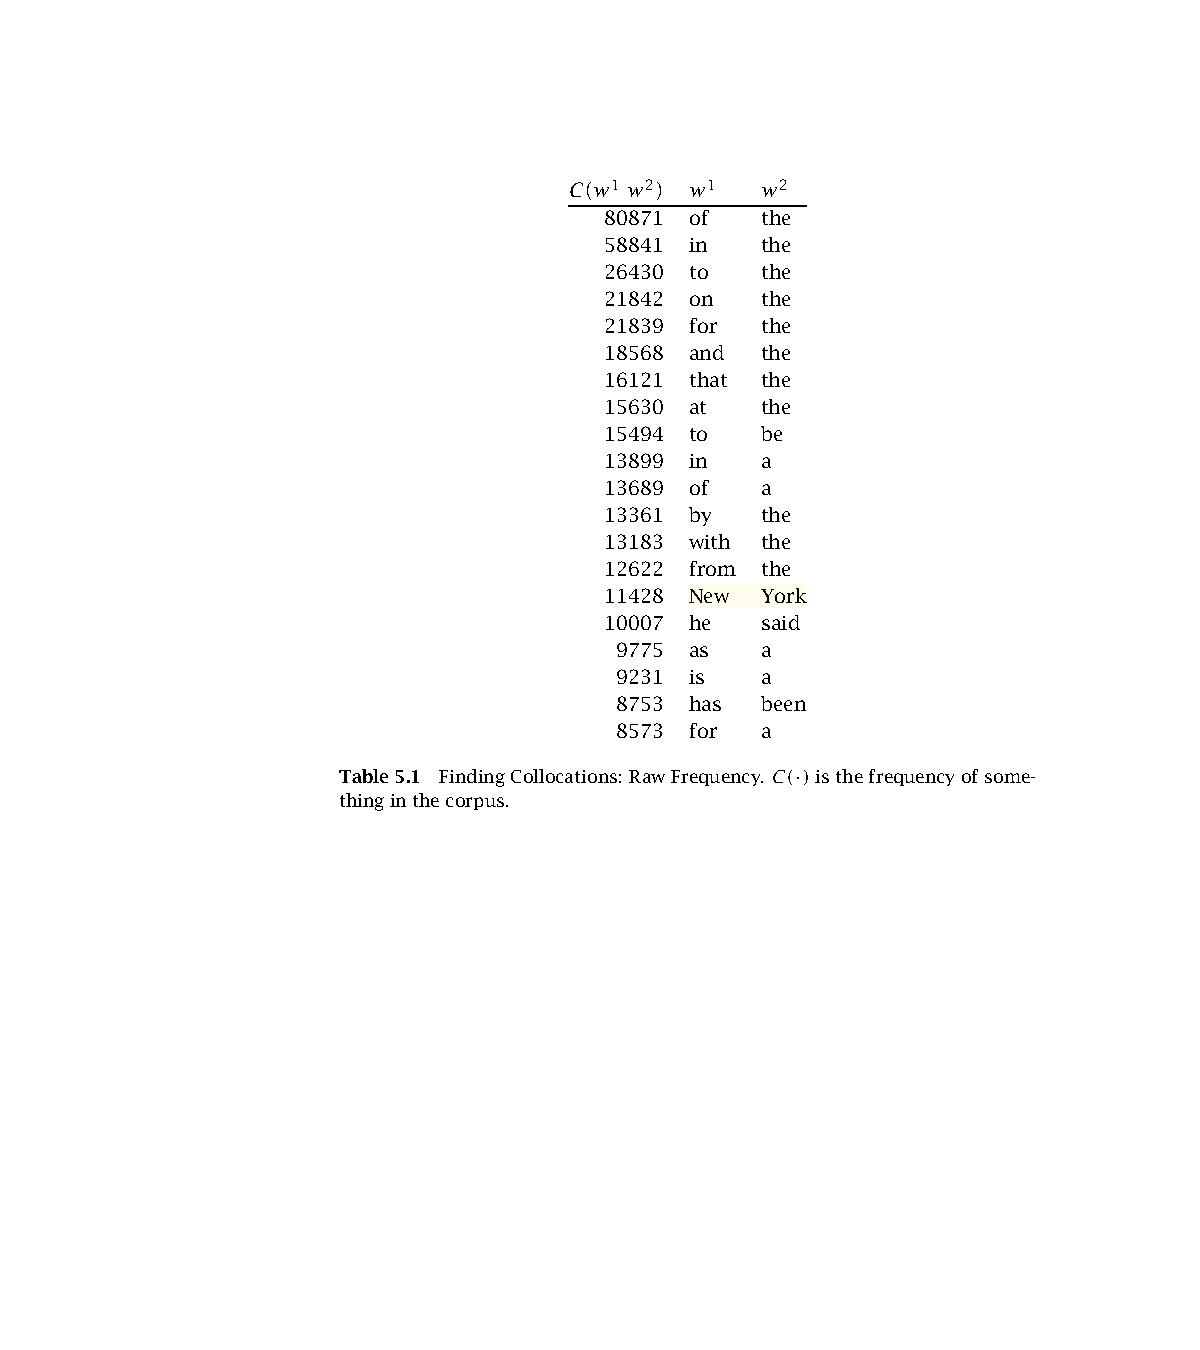
\includegraphics[height=.8\textheight]{MStable51.pdf}

  \footnotesize (from Manning and Sch\"utze, \emph{FSNLP}, Ch 5)
 \end{center}
\end{frame}

\begin{frame}
 \frametitle{Example}
 \begin{center}
  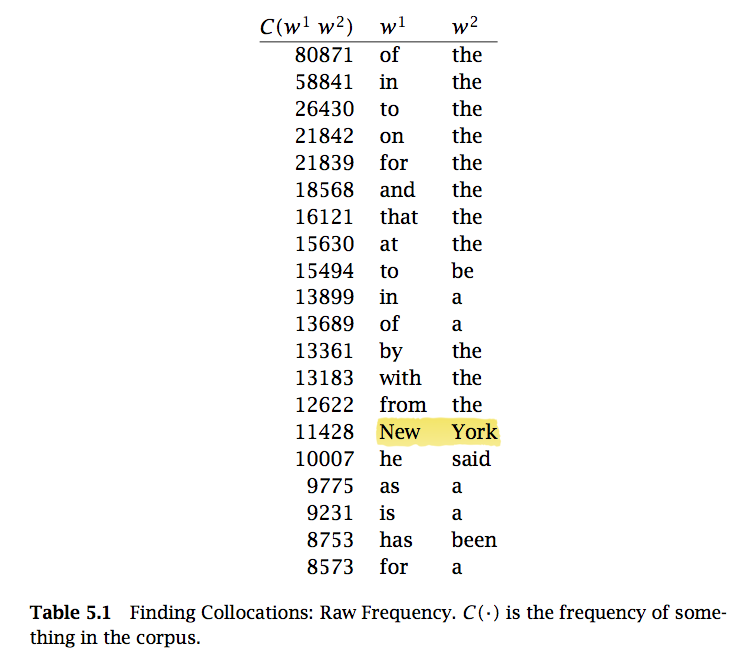
\includegraphics[height=.8\textheight]{MStable51b.png}

  \footnotesize (from Manning and Sch\"utze, \emph{FSNLP}, Ch 5)
 \end{center}
\end{frame}

\begin{frame}
 \frametitle{Contingency tables for bigrams}
 Tabulate every token against every other token as pairs, and compute
 for each token:
 \vspace*{1em}

 \centering
 \bgroup
 \def\arraystretch{1.5}%  1 is the default, change whatever you need
 \begin{tabular}[h]{|r|c|c|c|}
  \hline
               & token2   & $\neg$token2 & Totals   \\
  \hline
  token1       & $n_{11}$ & $n_{12}$     & $n_{1p}$ \\
  \hline
  $\neg$token1 & $n_{21}$ & $n_{22}$     & $n_{1p}$ \\[.5ex]
  \hline
  Totals       & $n_{p1}$ & $n_{p2}$     & $n_{pp}$ \\
  \hline
 \end{tabular}
 \egroup
\end{frame}

\begin{frame}
 \frametitle{Contingency tables for trigrams}
 \centering
 \bgroup
 \def\arraystretch{1.5}%  1 is the default, change whatever you need
 \begin{tabular}[h]{|r|c|c|c|c|c|}
  \hline
               &              & token3    & $\neg$token3 & Totals    \\
  \hline
  token1       & token2       & $n_{111}$ & $n_{112}$    & $n_{11p}$ \\
  \hline
  token1       & $\neg$token2 & $n_{121}$ & $n_{122}$    & $n_{12p}$ \\
  \hline
  $\neg$token1 & token2       & $n_{211}$ & $n_{212}$    & $n_{21p}$ \\
  \hline
  $\neg$token1 & $\neg$token2 & $n_{221}$ & $n_{222}$    & $n_{22p}$ \\[.5ex]
  \hline
  \multicolumn{2}{|r|}{Totals}    &  $n_{pp1}$ & $n_{pp2}$ & $n_{ppp}$ \\
  \hline
 \end{tabular}
 \egroup
\end{frame}


\begin{frame}
 \frametitle{computing the ``independence'' model}
 \vspace*{1em}
 \begin{itemize}
  \setlength{\itemsep}{2em}
  \item \alert{bigrams}
        \begin{align*}
         Pr(\mathsf{token1}, \mathsf{token2}) = Pr(\mathsf{token1})\/Pr(\mathsf{token2})
        \end{align*}
  \item \alert{trigrams}
        \begin{align*}
         Pr(\mathsf{t1}, \mathsf{t2}, \mathsf{t3}) & = Pr(\mathsf{t1})\/Pr(\mathsf{t2})\/Pr(\mathsf{t3}) \\
         Pr(\mathsf{t1}, \mathsf{t2}, \mathsf{t3}) & = Pr(\mathsf{t1}, \mathsf{t2})\/Pr(\mathsf{t3})     \\
         Pr(\mathsf{t1}, \mathsf{t2}, \mathsf{t3}) & = Pr(\mathsf{t1})\/Pr(\mathsf{t2})\/Pr(\mathsf{t3}) \\
         Pr(\mathsf{t1}, \mathsf{t2}, \mathsf{t3}) & = Pr(\mathsf{t1}, \mathsf{t3})\/Pr(\mathsf{t2})
        \end{align*}

 \end{itemize}
\end{frame}

\begin{frame}
 \frametitle{more independence models}
 \begin{itemize}
  \setlength{\itemsep}{2em}
  \item for 4-grams, there are 14 independence models
        \pause
  \item generally: the number equals the \emph{Bell number}
        less one, where the Bell number $B_n$ can be computed recursively as:
        \begin{align*}
         B_{n+1} & = \sum_{k=0}^n \binom{n}{k} B_k
        \end{align*}
        \pause \item but most of these are of limited relevance in collocation
        mining, as they subsume elements of earlier collocations
 \end{itemize}
\end{frame}



\begin{frame}
 \frametitle{statistical association measures}
 where $m_{ij}$ represents the cell frequency expected according to independence:
 \vspace*{1em}
 \begin{description}
  \setlength{\itemsep}{2em}
  \item[$G^2$] likelihood ratio statistic, computed as:
  \begin{align}
   2 * \sum_i \sum_j ( n_{ij} * log \frac{n_{ij}}{m_{ij}} )
  \end{align}

  \item[$\chi^2$] Pearson's $\chi^2$ statistic, computed as:
  \begin{align}
   \sum_i \sum_j \frac{(n_{ij} - m_{ij})^2}{m_{ij}}
  \end{align}
 \end{description}
\end{frame}

\begin{frame}
 \frametitle{statistical association measures (cont.)}
 \begin{description}
  \setlength{\itemsep}{2em}
  \item[pmi] point-wise mutual information score, computed as log\@$n_{11}/m_{11}$
  \item[dice] the Dice coefficient, computed as
  \begin{align}
   \frac{n_{11}}{n_{1.} + n_{.1}}
  \end{align}
 \end{description}
\end{frame}



% \begin{frame}
%   \frametitle{Detecting collocations: Constructing the association table}
%     \begin{center}
%     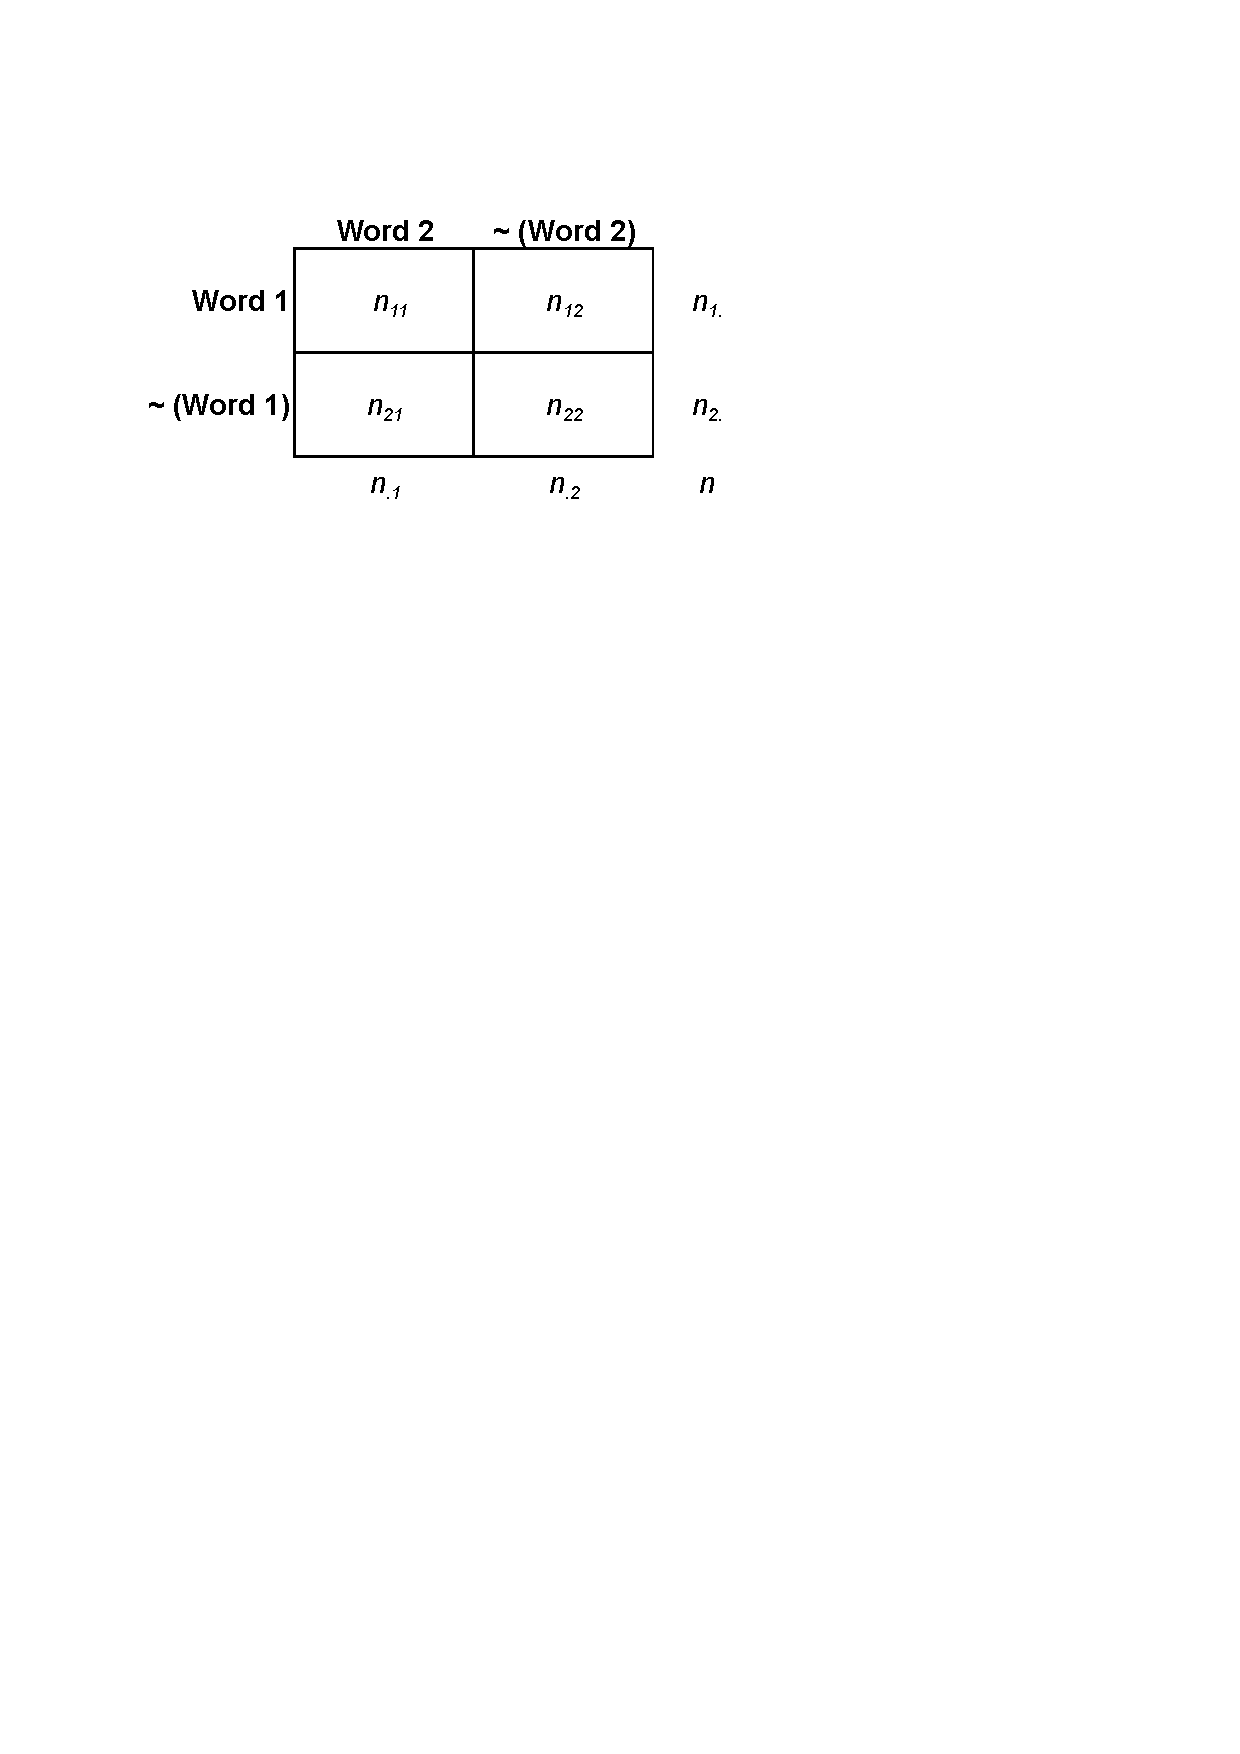
\includegraphics[width=.6\textwidth]{bigramtable.pdf}
%     where:
%     \begin{description}
%     \item[$n_{ij}$] are observed counts
%     \item[$n_{i.}, n_{.j}$] are row, column marginals
%     \item[$n$] is total token count
%     \item[$m_{ij} = \frac{n_{i.} n_{.j}}{n}$] is an \emph{expected} count
%       under the independence model
%     \end{description}
%     \end{center}

% \end{frame}

% \begin{frame}
%   \frametitle{Method 1: Pearson's chi-squared statistic}
%     \begin{center}
%     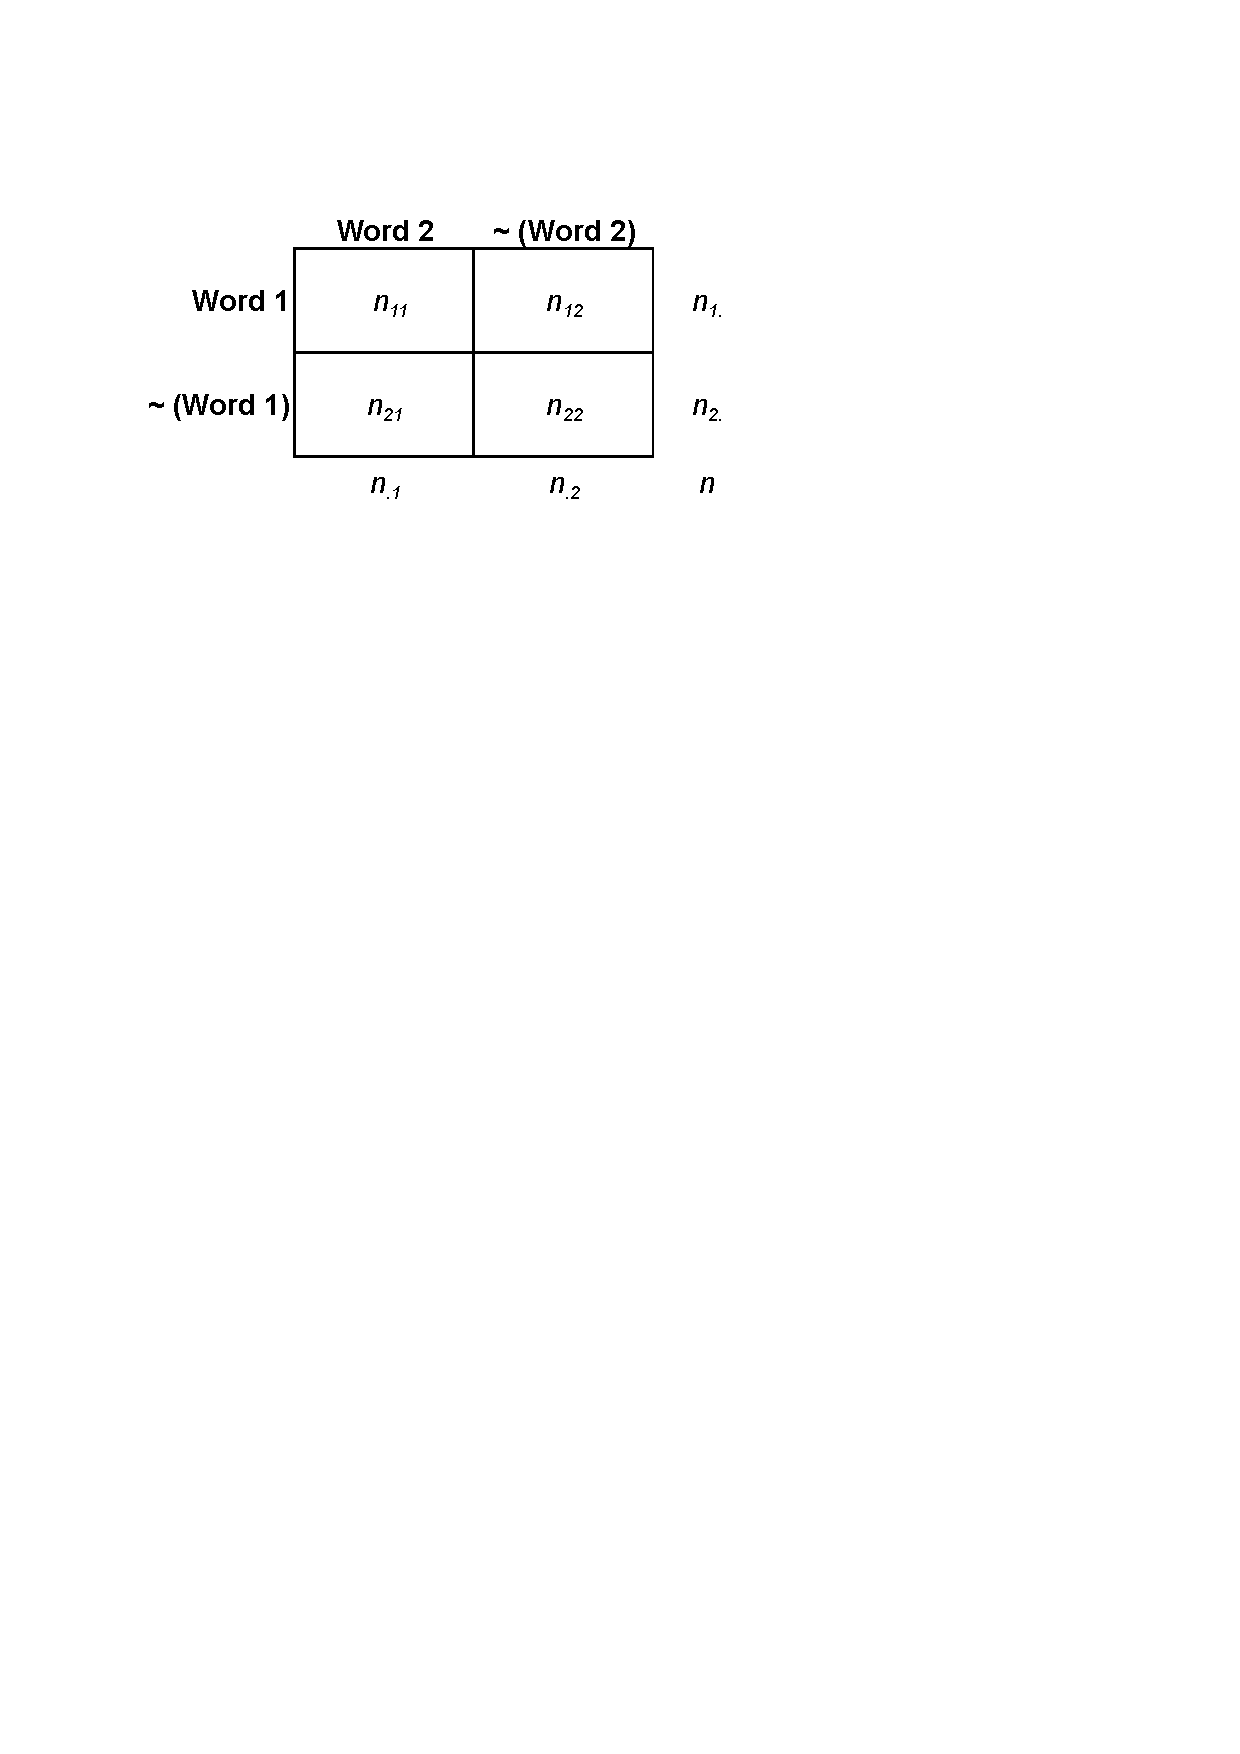
\includegraphics[width=.6\textwidth]{bigramtable.pdf}

%     \begin{equation*}
%       X^2 = \sum_i \sum_j \frac{(n_{ij} - m_{ij})^2}{m_{ij}}
%     \end{equation*}
%     where $X \sim \chi^2$ with 1 d.f. [same as $(I-1)(J-1)$]

%     \end{center}

% \end{frame}


% \begin{frame}
%   \frametitle{Method 2: Likelihood ratio test (Dunning)}
%     \begin{center}
%     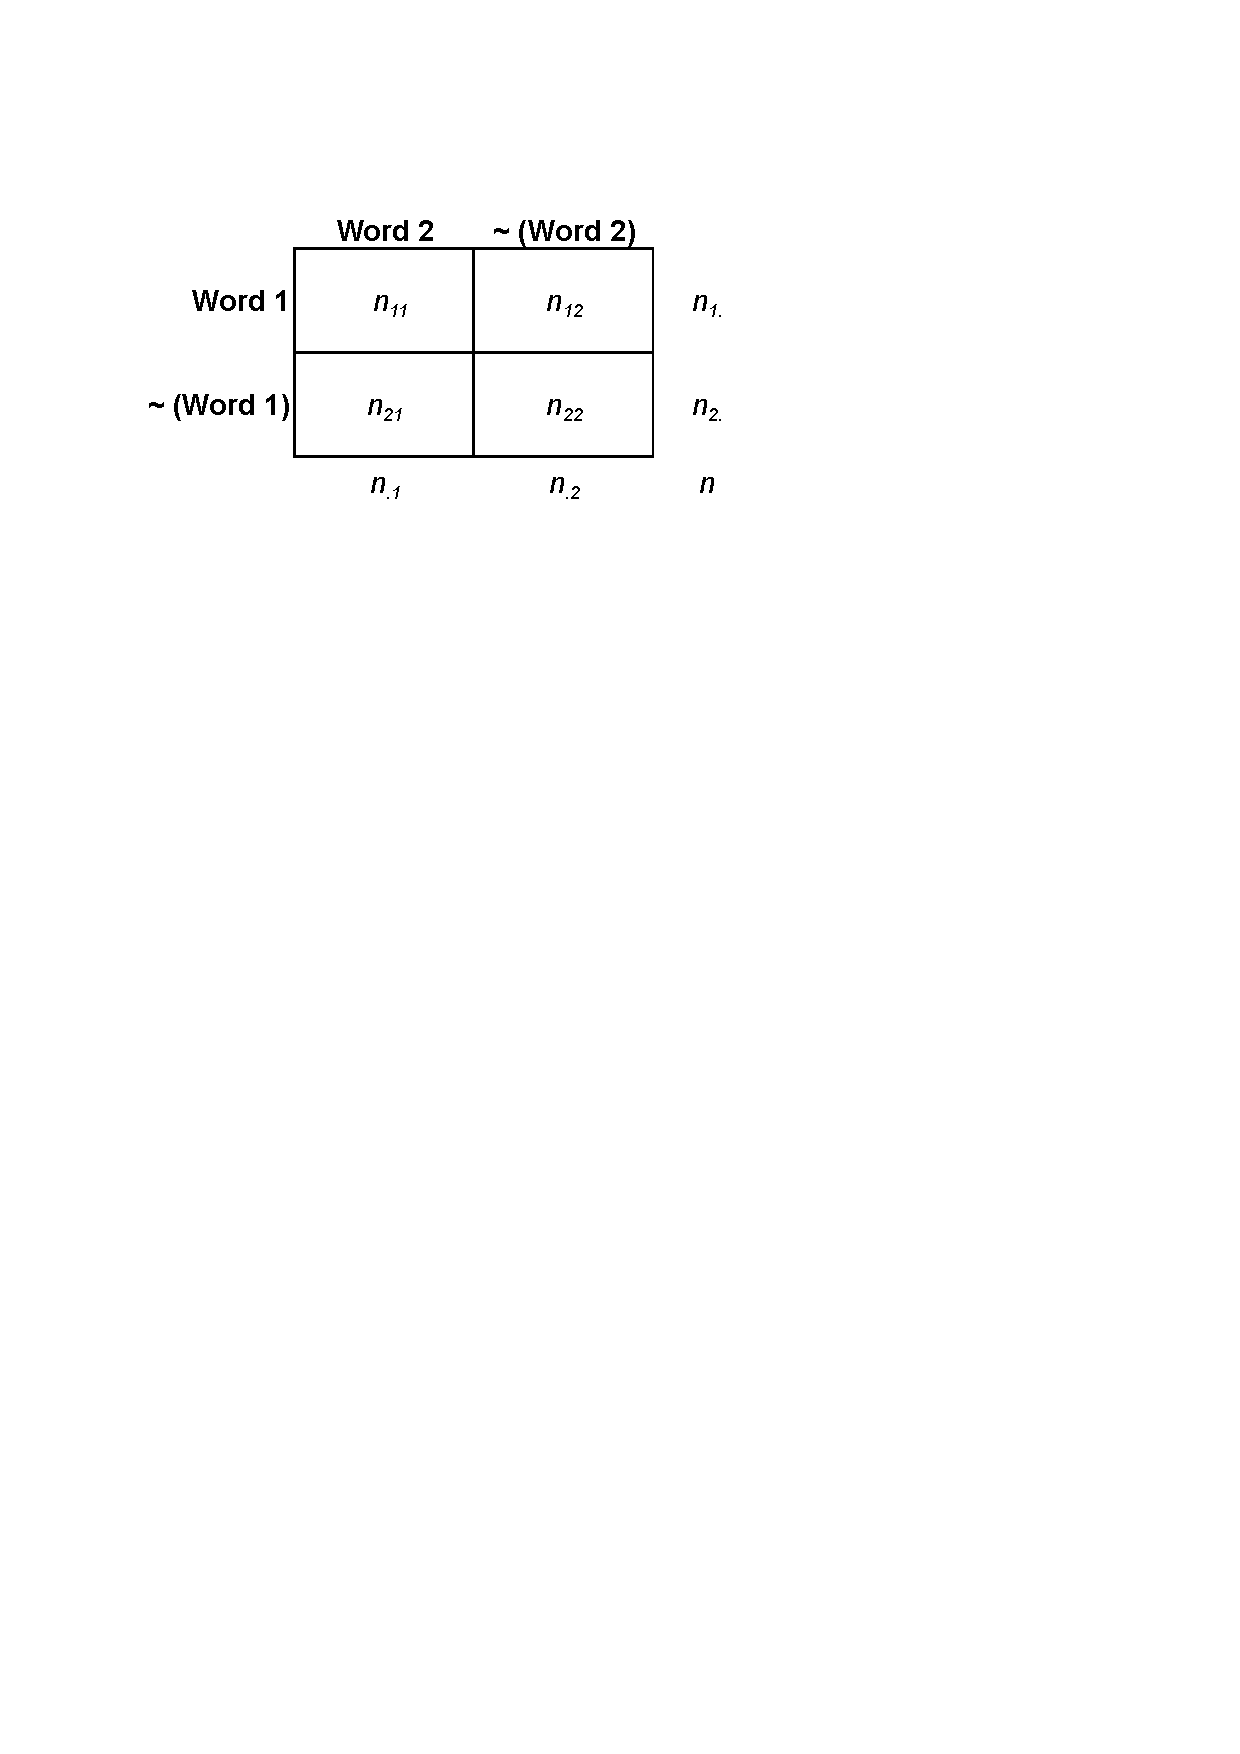
\includegraphics[width=.6\textwidth]{bigramtable.pdf}

%     \begin{equation*}
%       G^2 = 2 \sum_i \sum_j n_{ij} \ \mathrm{ln} \frac{n_{ij}}{m_{ij}}
%     \end{equation*}
%     where $G \sim \chi^2$ with 1 d.f. [same as $(I-1)(J-1)$]
%     \end{center}
% \end{frame}

% \begin{frame}
%   \frametitle{Generalization to trigrams}
%   \begin{center}
%     \begin{equation*}
%       G^2 = 2 \sum_i \sum_j \sum_k n_{ijk} \ \mathrm{ln} \frac{n_{ijk}}{m_{ijk}}
%     \end{equation*}
%   \end{center}

%     where
%     \begin{itemize}
%     \item $G \sim \chi^2$ with 1 d.f. [same as $(I-1)(J-1)(K-1)$]
%     \item $m_{ijk} = \frac{n_{i..} n_{.j.} n_{..k}}{n}$ is an \emph{expected} count
%       under the independence model
%     \item but the table of observed counts is slightly more complicated, as
%     is the calculation of two words dependence but independence of the
%     third -- see Bautin and Hart for details
%     \end{itemize}
% \end{frame}


% \begin{frame}
%   \frametitle{Other methods}
%     % \begin{center}
%     % 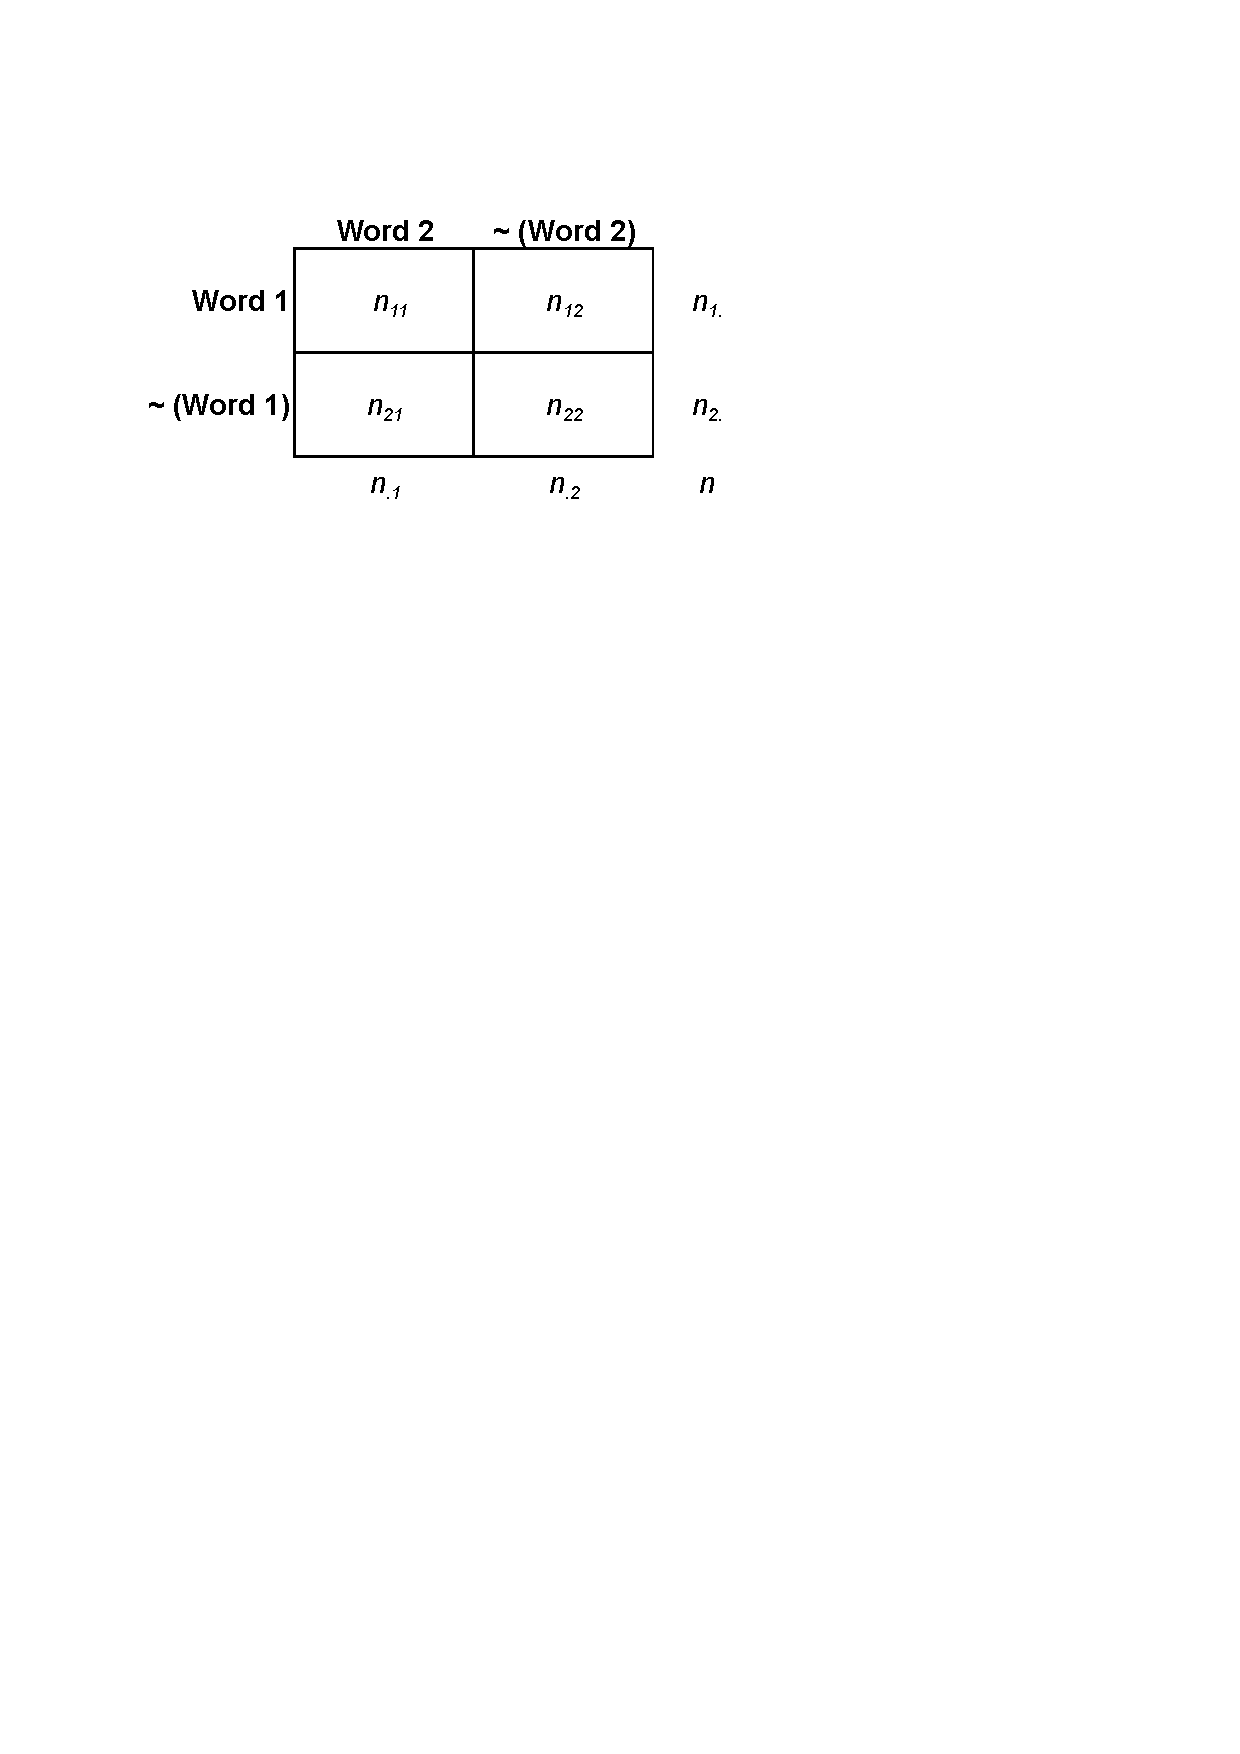
\includegraphics[width=.6\textwidth]{bigramtable.pdf}
%     \begin{itemize}
%     \item $t$-tests of frequencies (but assumes normality)
%     \item mutual information, pointwise mutual information
%     \item Pearson exact tests
%     \item Many more: see Pecina (2005) for an exhaustive(ing) listing
%     \end{itemize}
%     % \end{center}
% \end{frame}

\begin{frame}
 \frametitle{Augmenting collocation detection with additional
 information}
 \begin{itemize}
  \item Use parts of speech information
        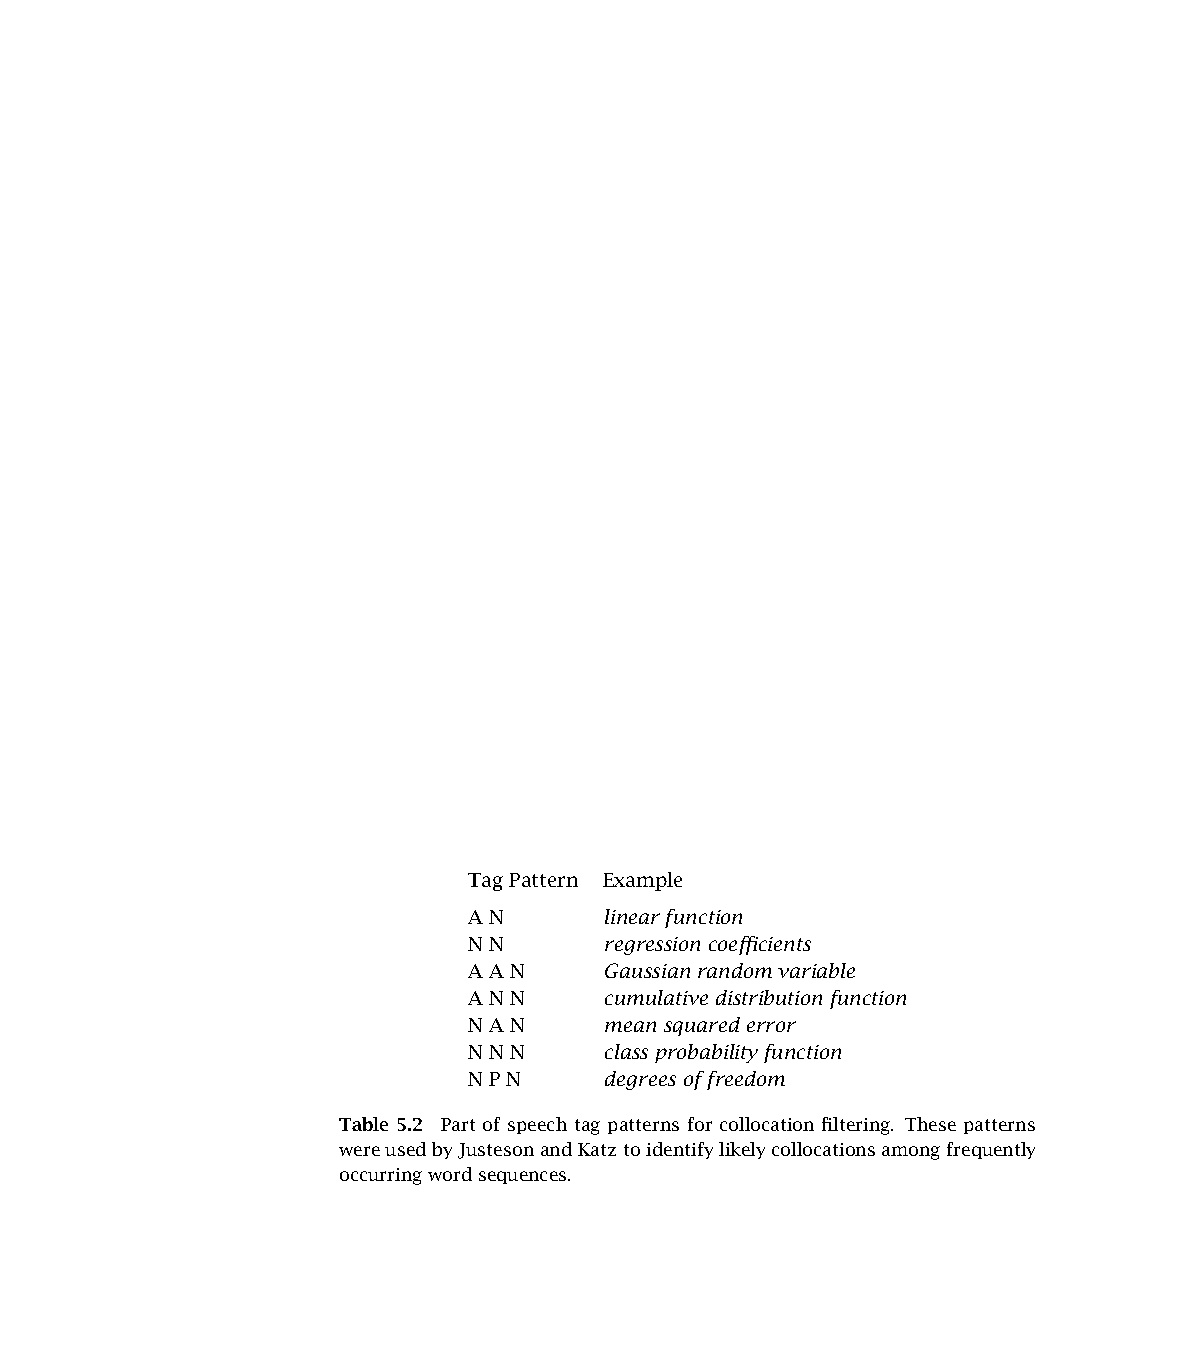
\includegraphics[width=.9\textwidth]{MStable52.pdf}
  \item other (machine prediction) tools
 \end{itemize}
\end{frame}

\begin{frame}[fragile]
 \frametitle{Named Entity recognition}
 \scriptsize
 \begin{verbatim}
   > sp <- spacy_parse(txt, tag = TRUE)
   > entity_consolidate(sp)
      doc_id sentence_id token_id          token          lemma    pos    tag entity_type
   1   text1           1        1  Pierre_Vinken  pierre_vinken ENTITY ENTITY      PERSON
   2   text1           1        2              ,              ,  PUNCT      ,
   3   text1           1        3   61_years_old    61_year_old ENTITY ENTITY        DATE
   4   text1           1        4              ,              ,  PUNCT      ,
   5   text1           1        5           will           will   VERB     MD
   6   text1           1        6           join           join   VERB     VB
   7   text1           1        7            the            the    DET     DT
   8   text1           1        8          board          board   NOUN     NN
   9   text1           1        9             as             as    ADP     IN
   10  text1           1       10              a              a    DET     DT
   11  text1           1       11   nonexecutive   nonexecutive    ADJ     JJ
   12  text1           1       12     \n             \n          SPACE     SP
   13  text1           1       13       director       director   NOUN     NN
   14  text1           1       14        Nov._29        nov._29 ENTITY ENTITY        DATE
   15  text1           1       15              .              .  PUNCT      .
  \end{verbatim}
\end{frame}





\end{document}



\section{Inference/Reporting}

\begin{frame}
 \frametitle{Inference and Reporting}
 \begin{itemize}
  \setlength{\itemsep}{2ex}
  \item This involves drawing conclusions from the research, and these
        conclusions will depend on the \emph{validity} established by the
        research design
  \item Reporting means communicating the results in a clear and
        relevant fashion.  (This can be challenging -- see for instance
        the Schonhardt-Bailey article.)
  \item No iron-clad rules here -- use your discretion as applied to a
        particular case
 \end{itemize}
\end{frame}


\begin{frame}
 \frametitle{Summarizing: Example}
 \begin{figure}
  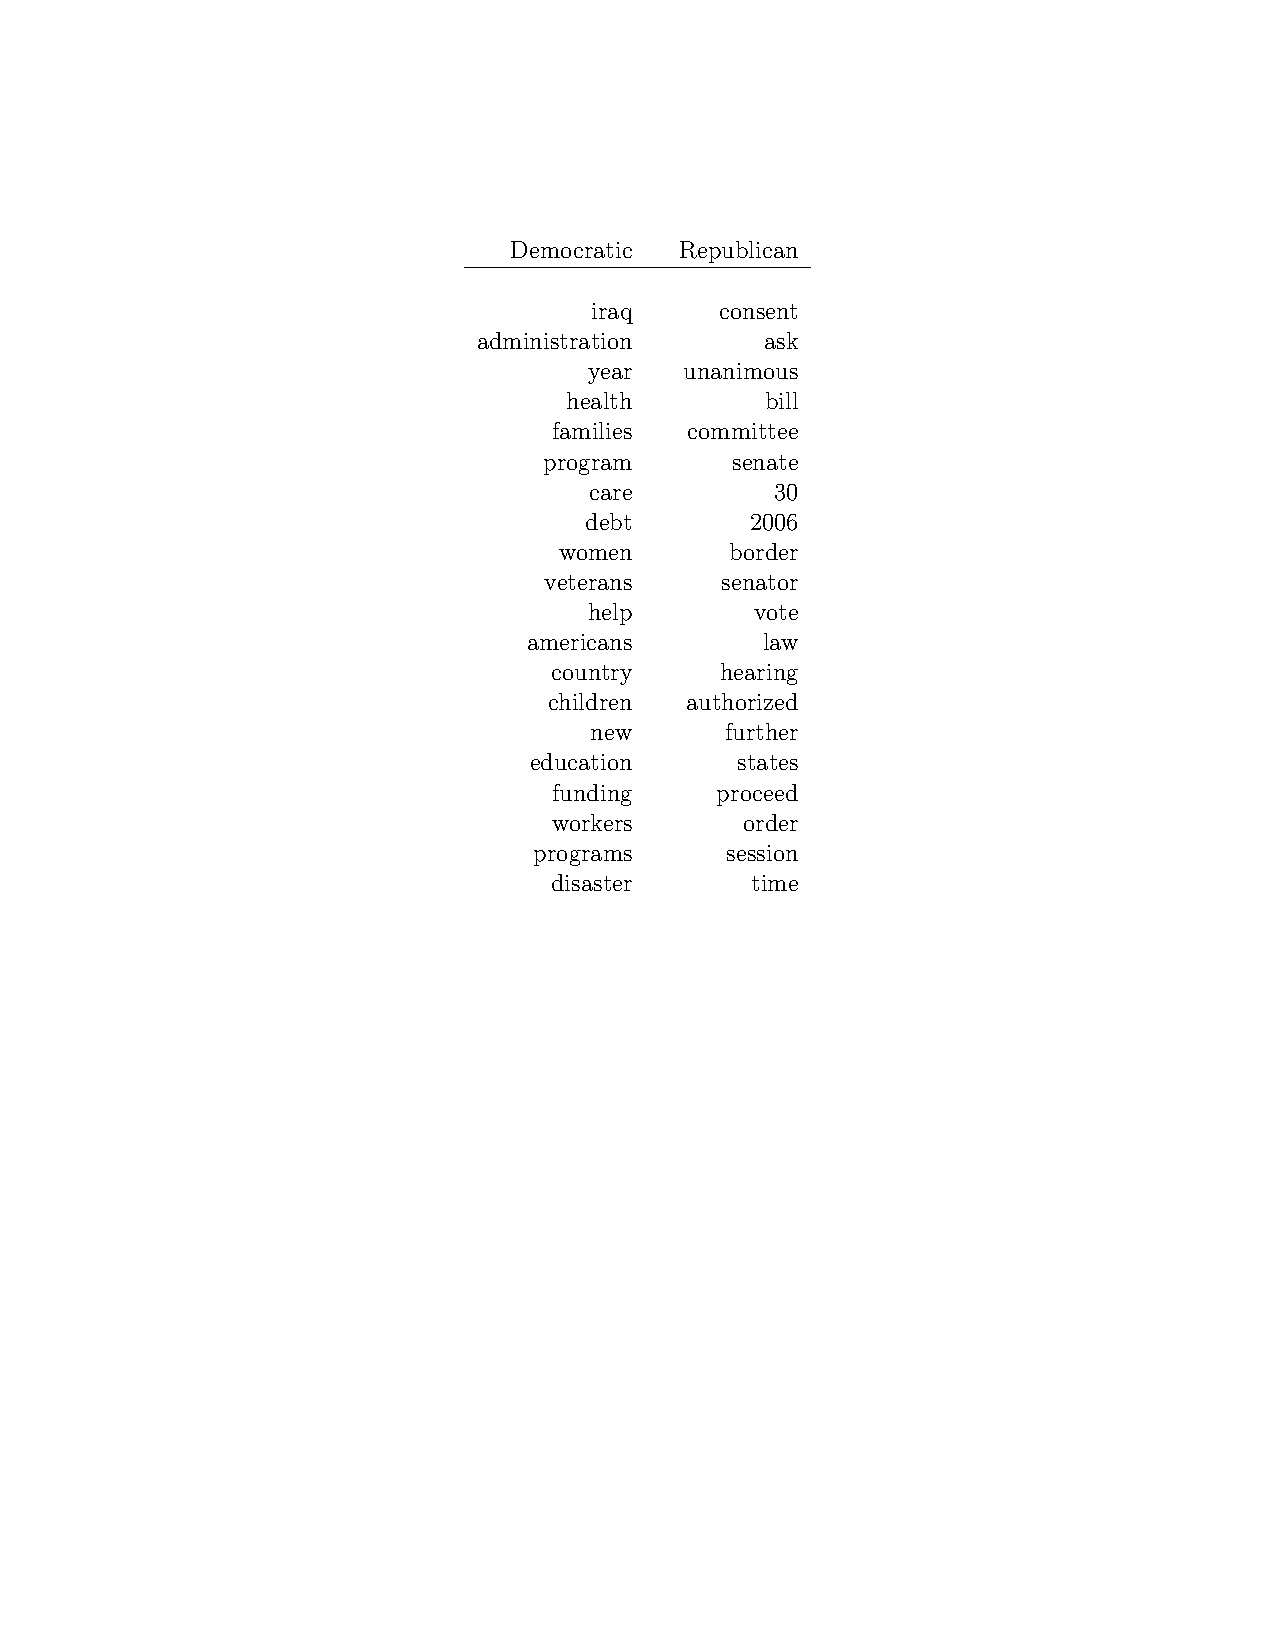
\includegraphics[height=7cm]{top20demrepwords.pdf}
 \end{figure}
 {\footnotesize Top 20 Democratic and Republican words from the 2006 US Senate
 (source: Nicholas Beauchamp 2008)}
\end{frame}

\begin{frame}
 \frametitle{LIWC Example}
 \begin{itemize}
  \item From an application of the Linguistic Inquiry and Word Count
        dictionary to texts by Al Zawahiri and Bin Laden, benchmarked
        against a general corpus
        \center 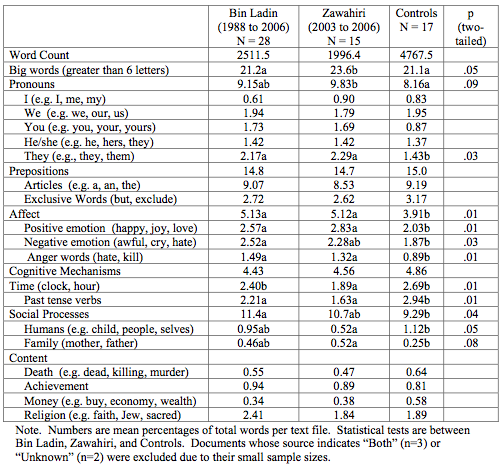
\includegraphics[width=7.5cm]{binladen.png}
 \end{itemize}
\end{frame}



\begin{frame}
 \frametitle{Graphical Methods: Example}
 \begin{itemize}
  \item From a uni-dimensional scaling model from a term-document
        matrix (Poisson scaling)
        \center 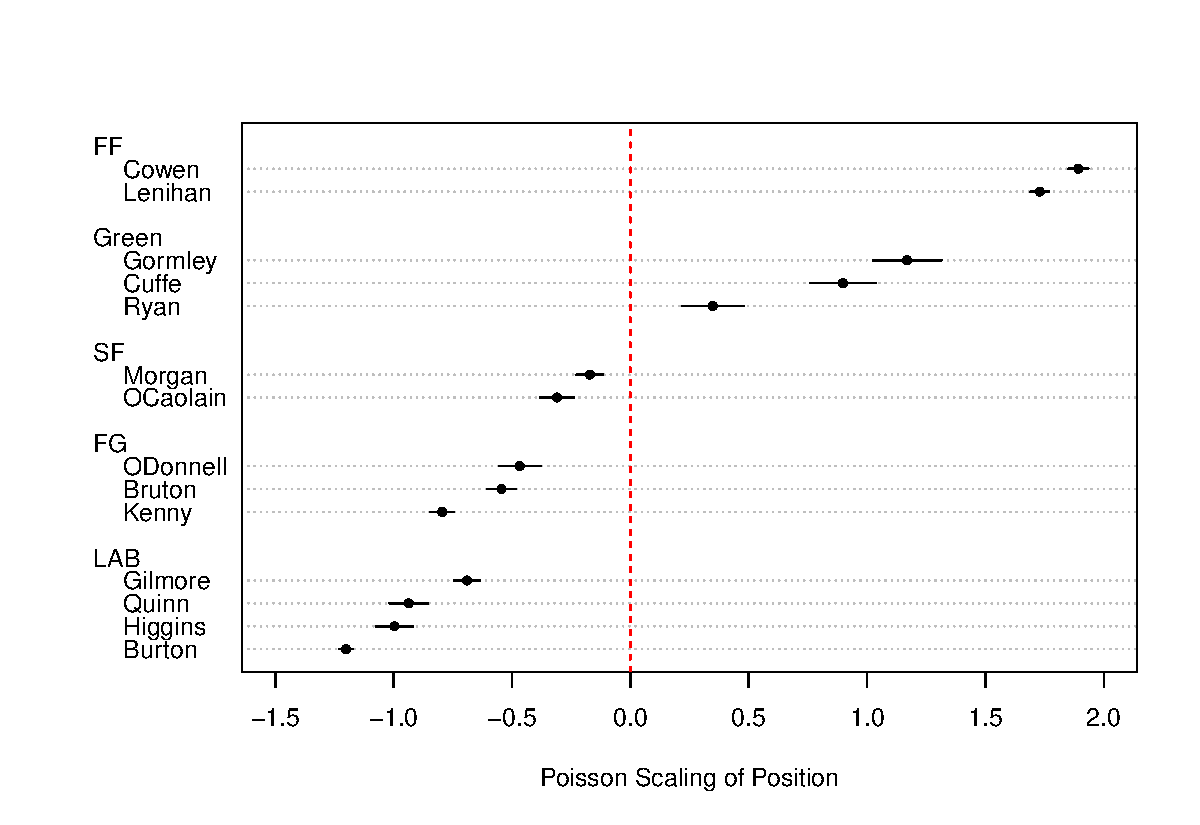
\includegraphics[width=10cm]{dotplot_wfscaled.pdf}
 \end{itemize}
\end{frame}

\begin{frame}
 \frametitle{No confidence debate speeches (Wordscores)}
 \center 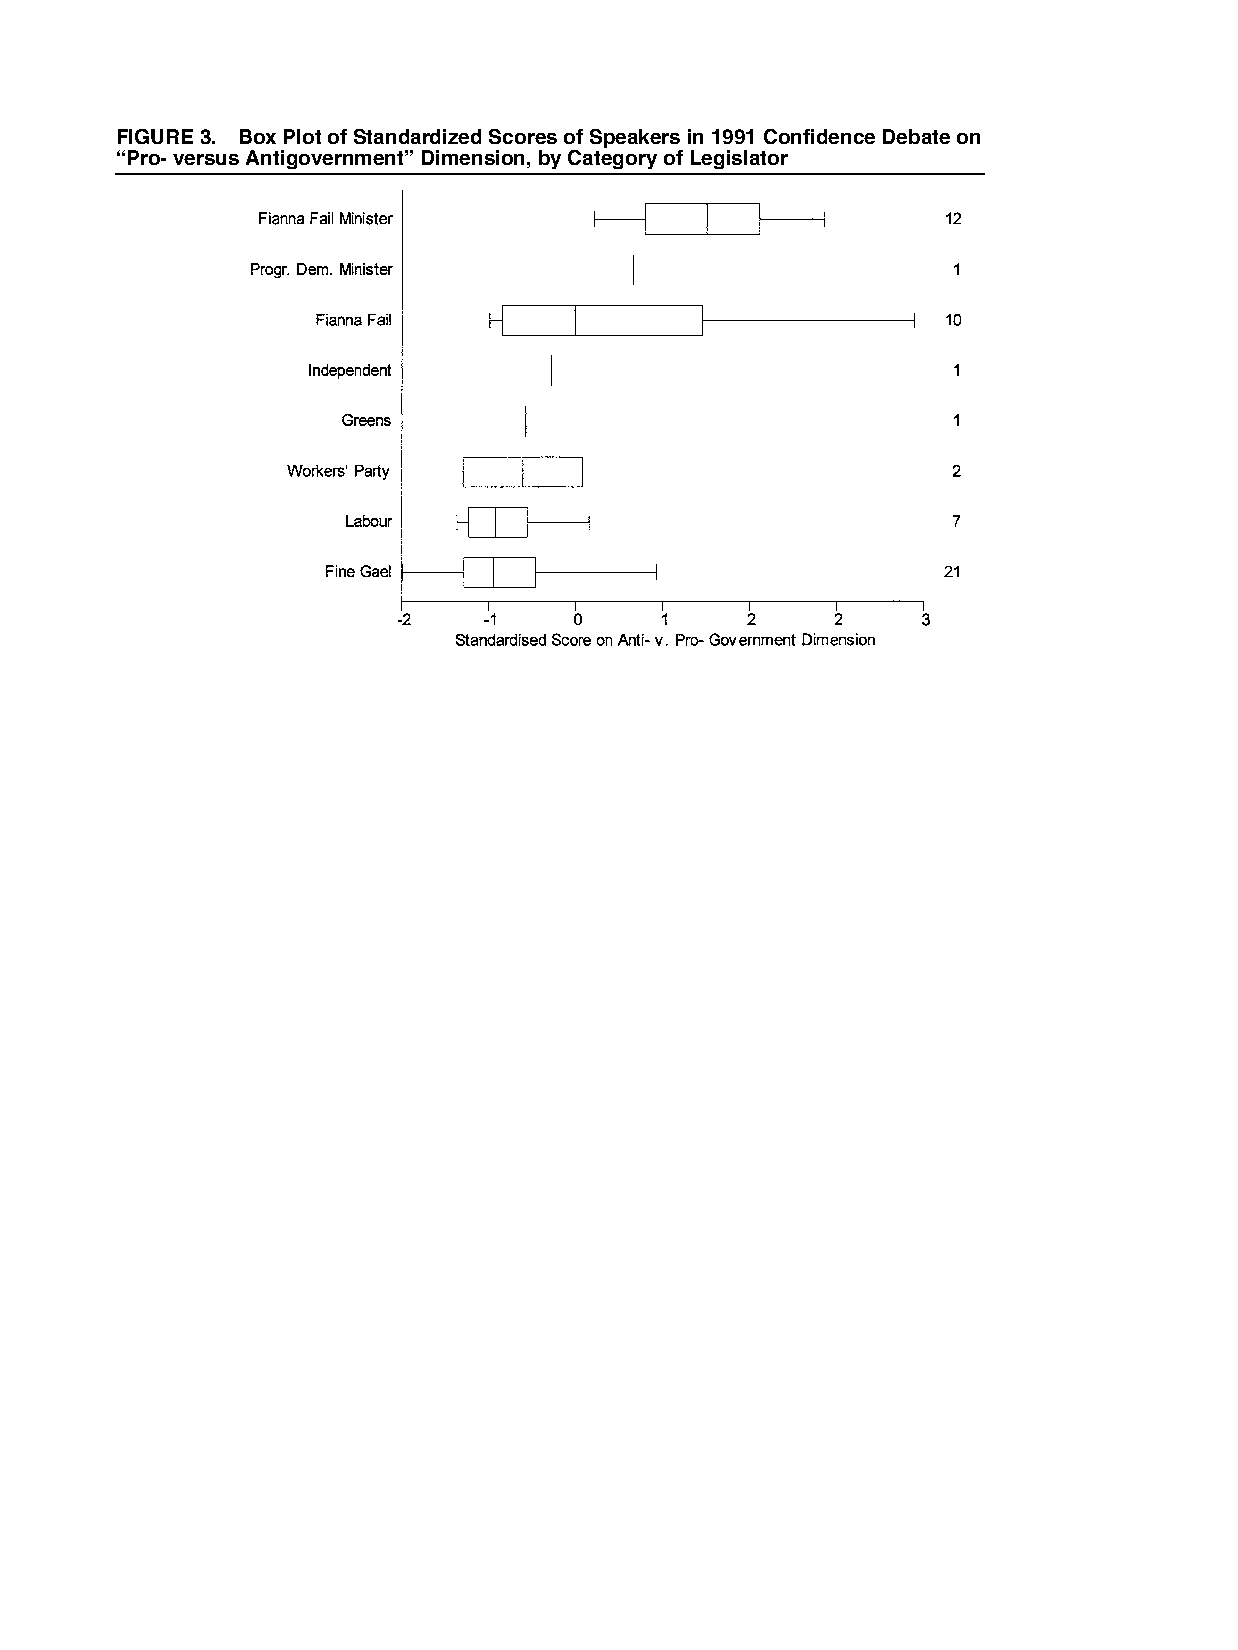
\includegraphics[width=10cm]{noconf.pdf}

 {\footnotesize (from Benoit and Laver, \emph{Irish Political Studies} 2002)}
\end{frame}


\begin{frame}
 \frametitle{Government v. Opposition in yearly budget debates}
 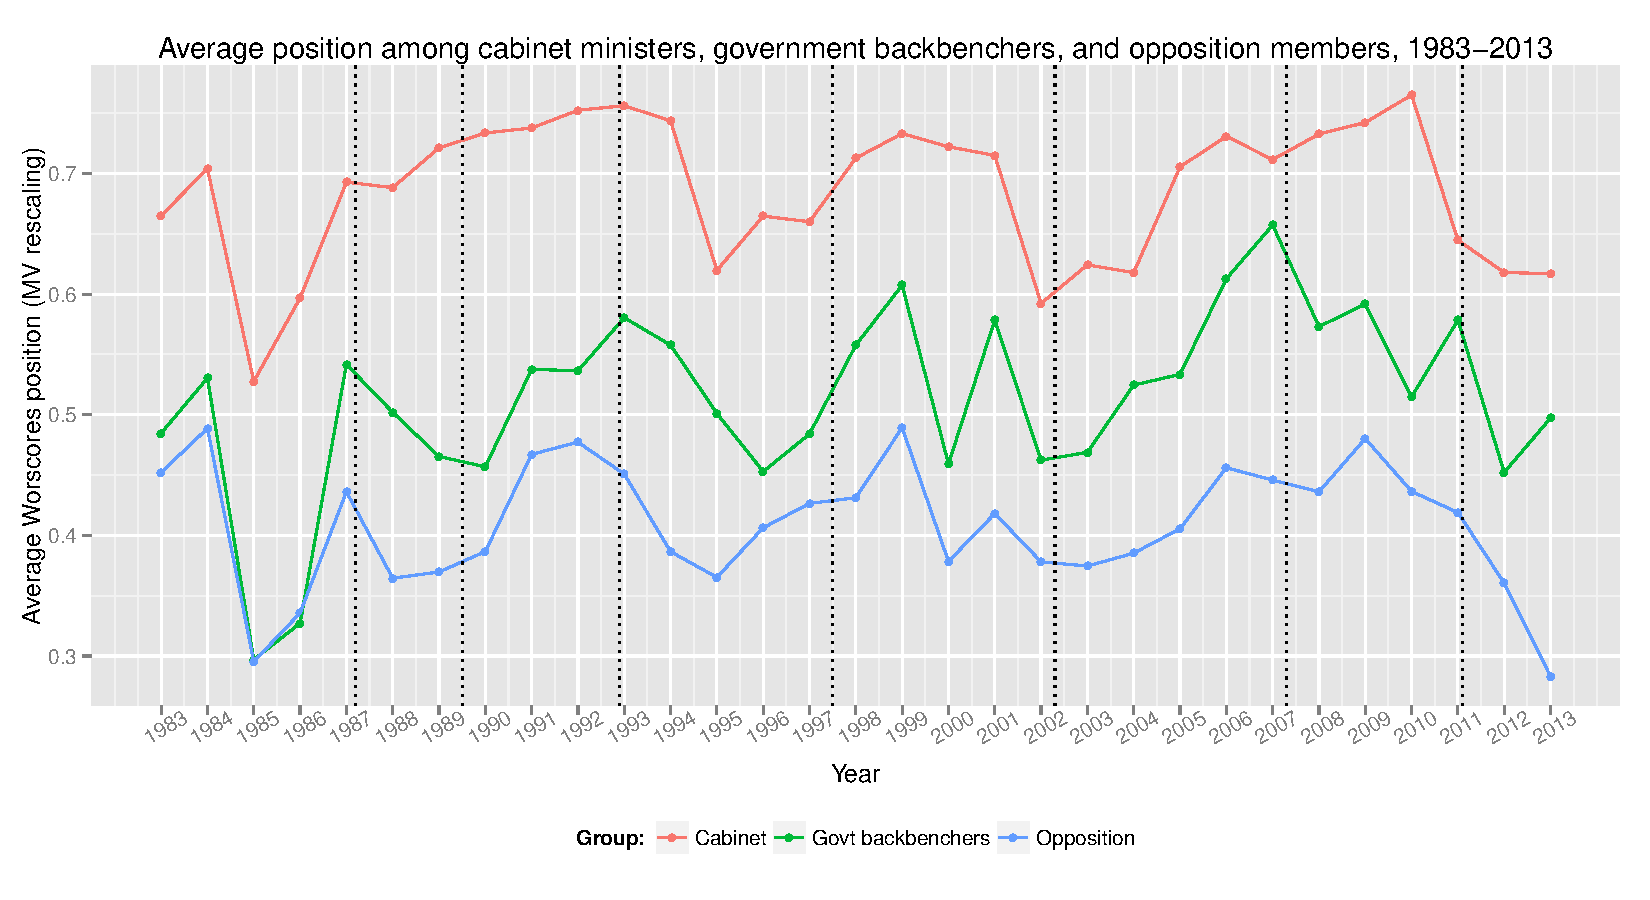
\includegraphics[width=\textwidth]{avg_positions_over_time.pdf}

 {\footnotesize (from Herzog and Benoit EPSA 2013)}
\end{frame}


\begin{frame}
 \frametitle{Comparing Texts on the Basis of Quantitative
 Information}
 \begin{center}
  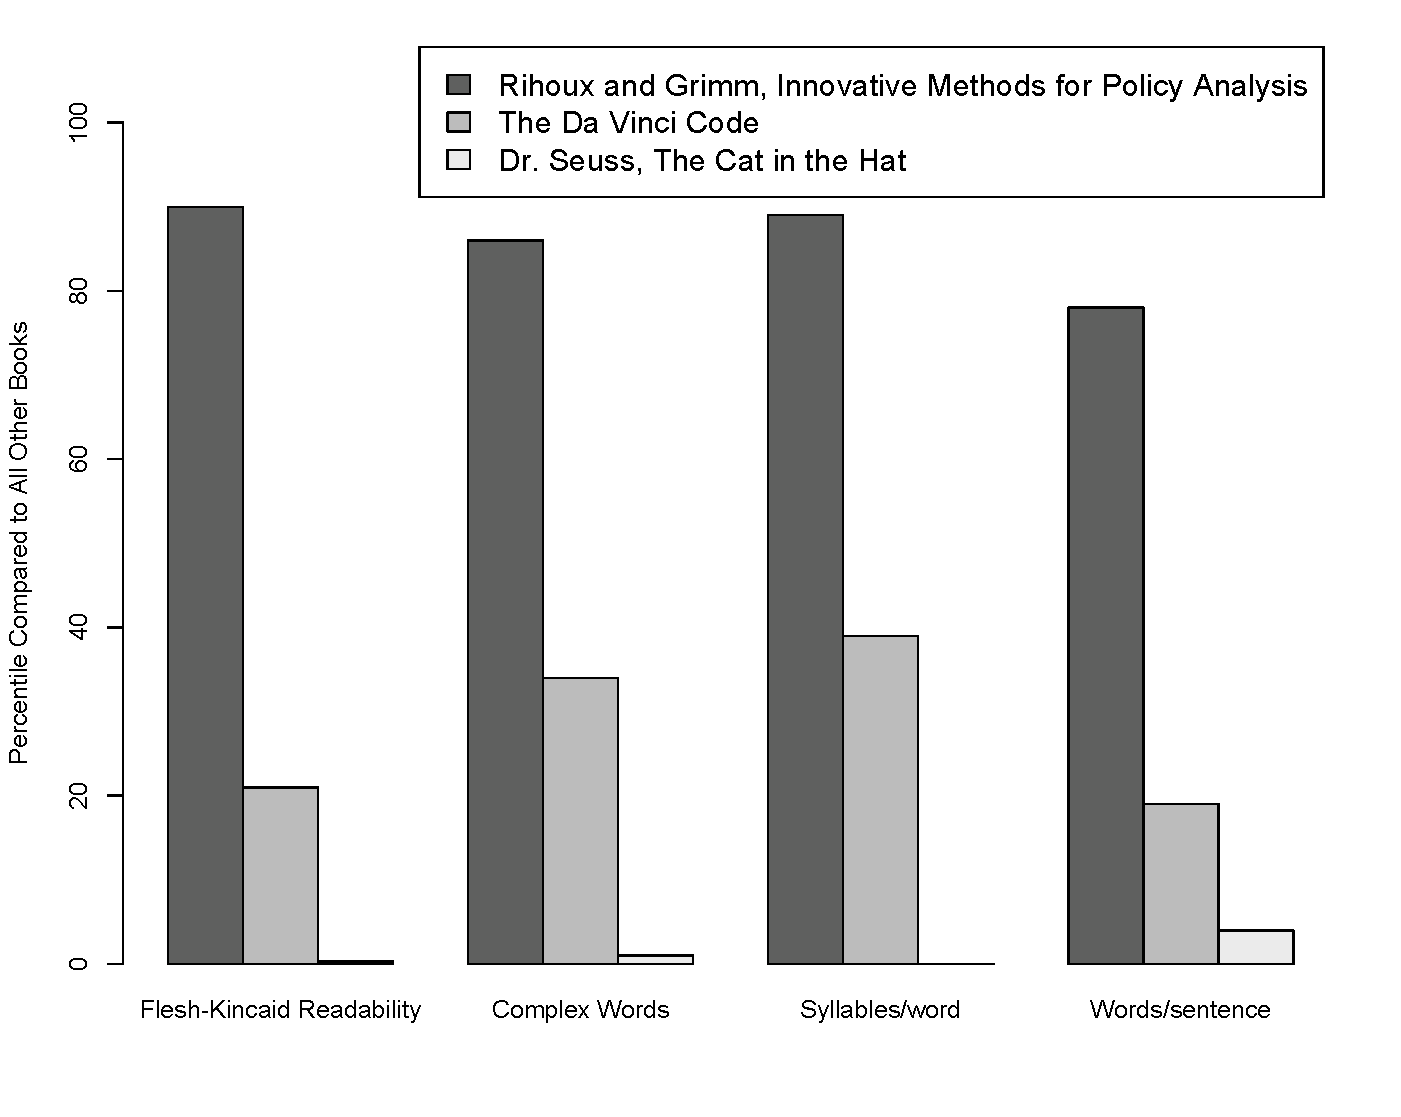
\includegraphics[width=10cm]{comparebooks.pdf}
 \end{center}
\end{frame}

\begin{frame}
 \frametitle{Applied to political texts}
 \alert{\hspace*{1.5cm} Bush's second inaugural address:}
 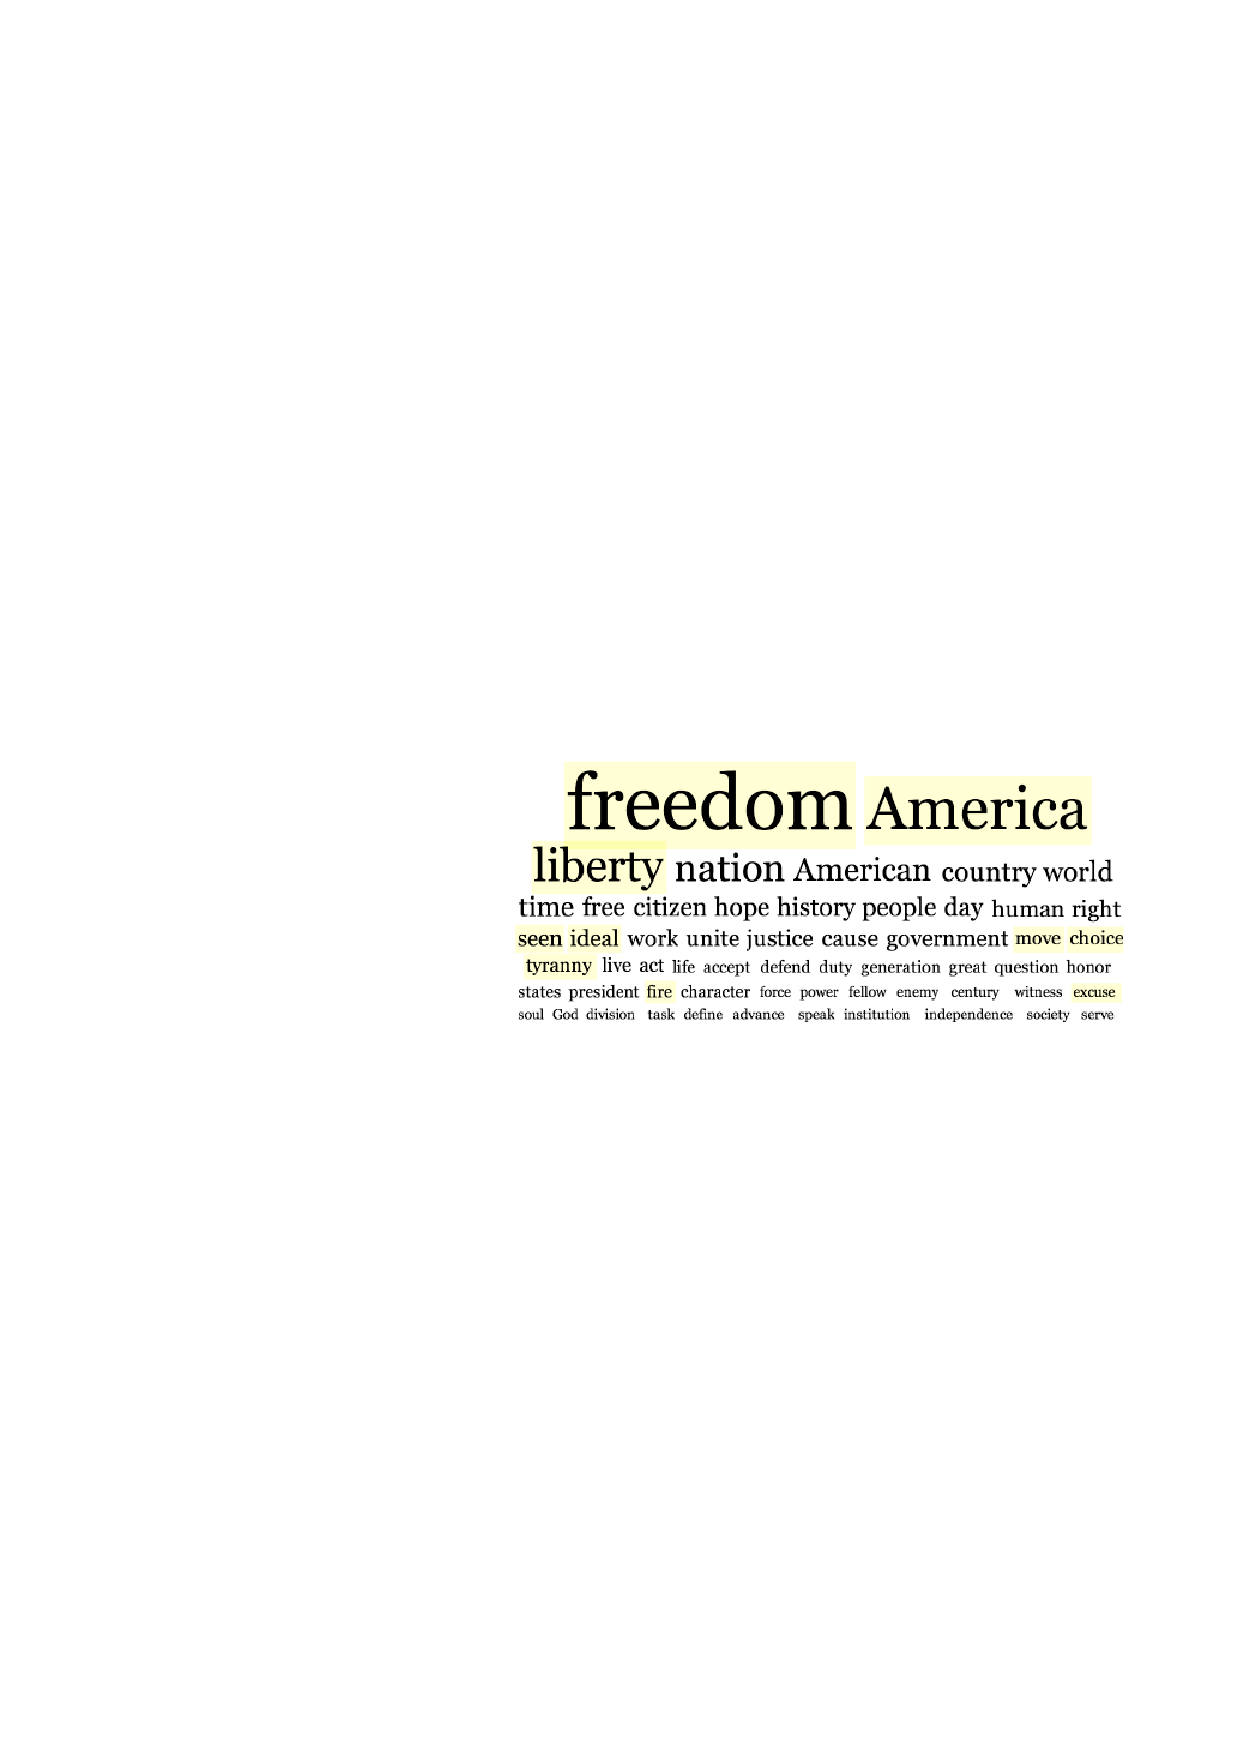
\includegraphics[width=7.8cm]{concordanceBush2.pdf}
 \begin{flushright}
  \alert{Obama's inaugural address: \hspace*{1.5cm}}
  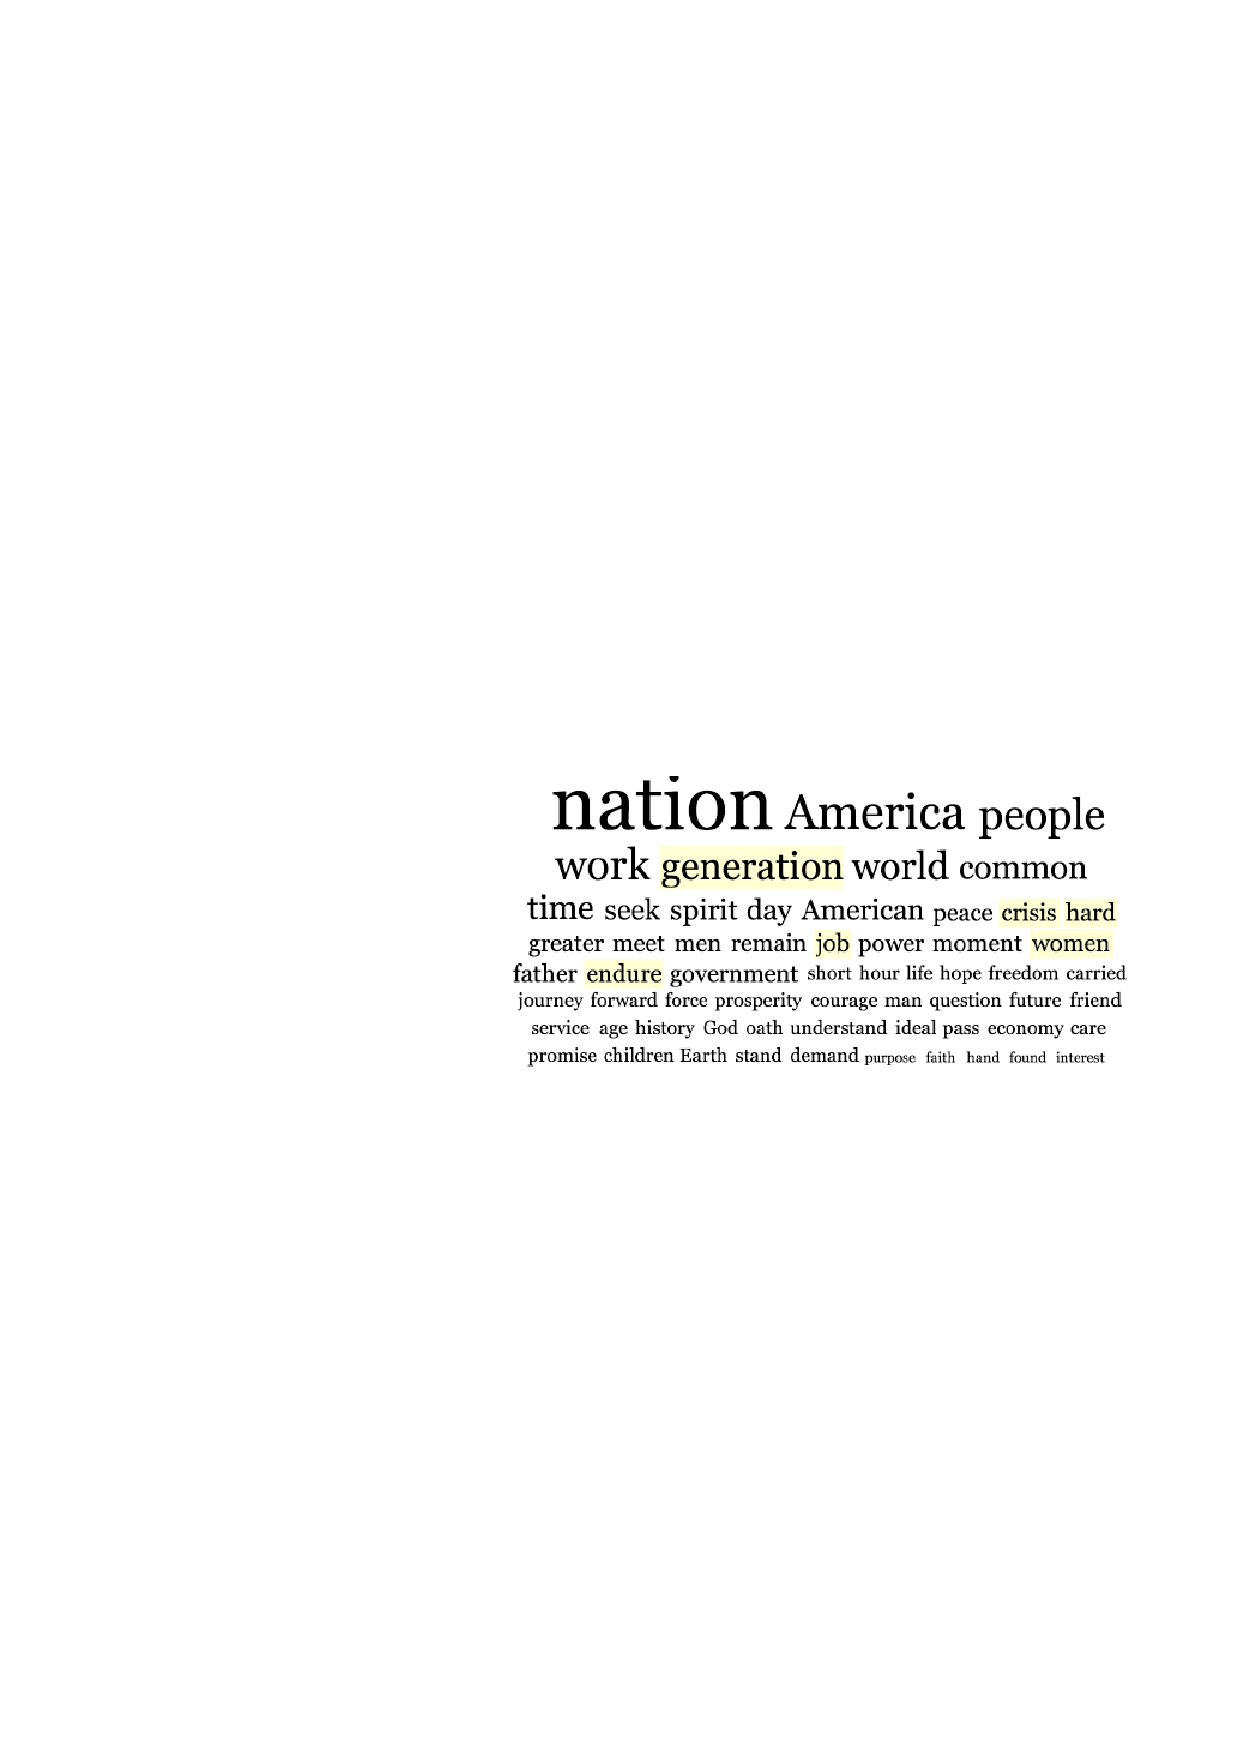
\includegraphics[width=7.8cm]{concordanceObama.pdf}
 \end{flushright}
\end{frame}

\begin{frame}
 \frametitle{Obama's Inaugural Speech in Wordle}
 \begin{center}
  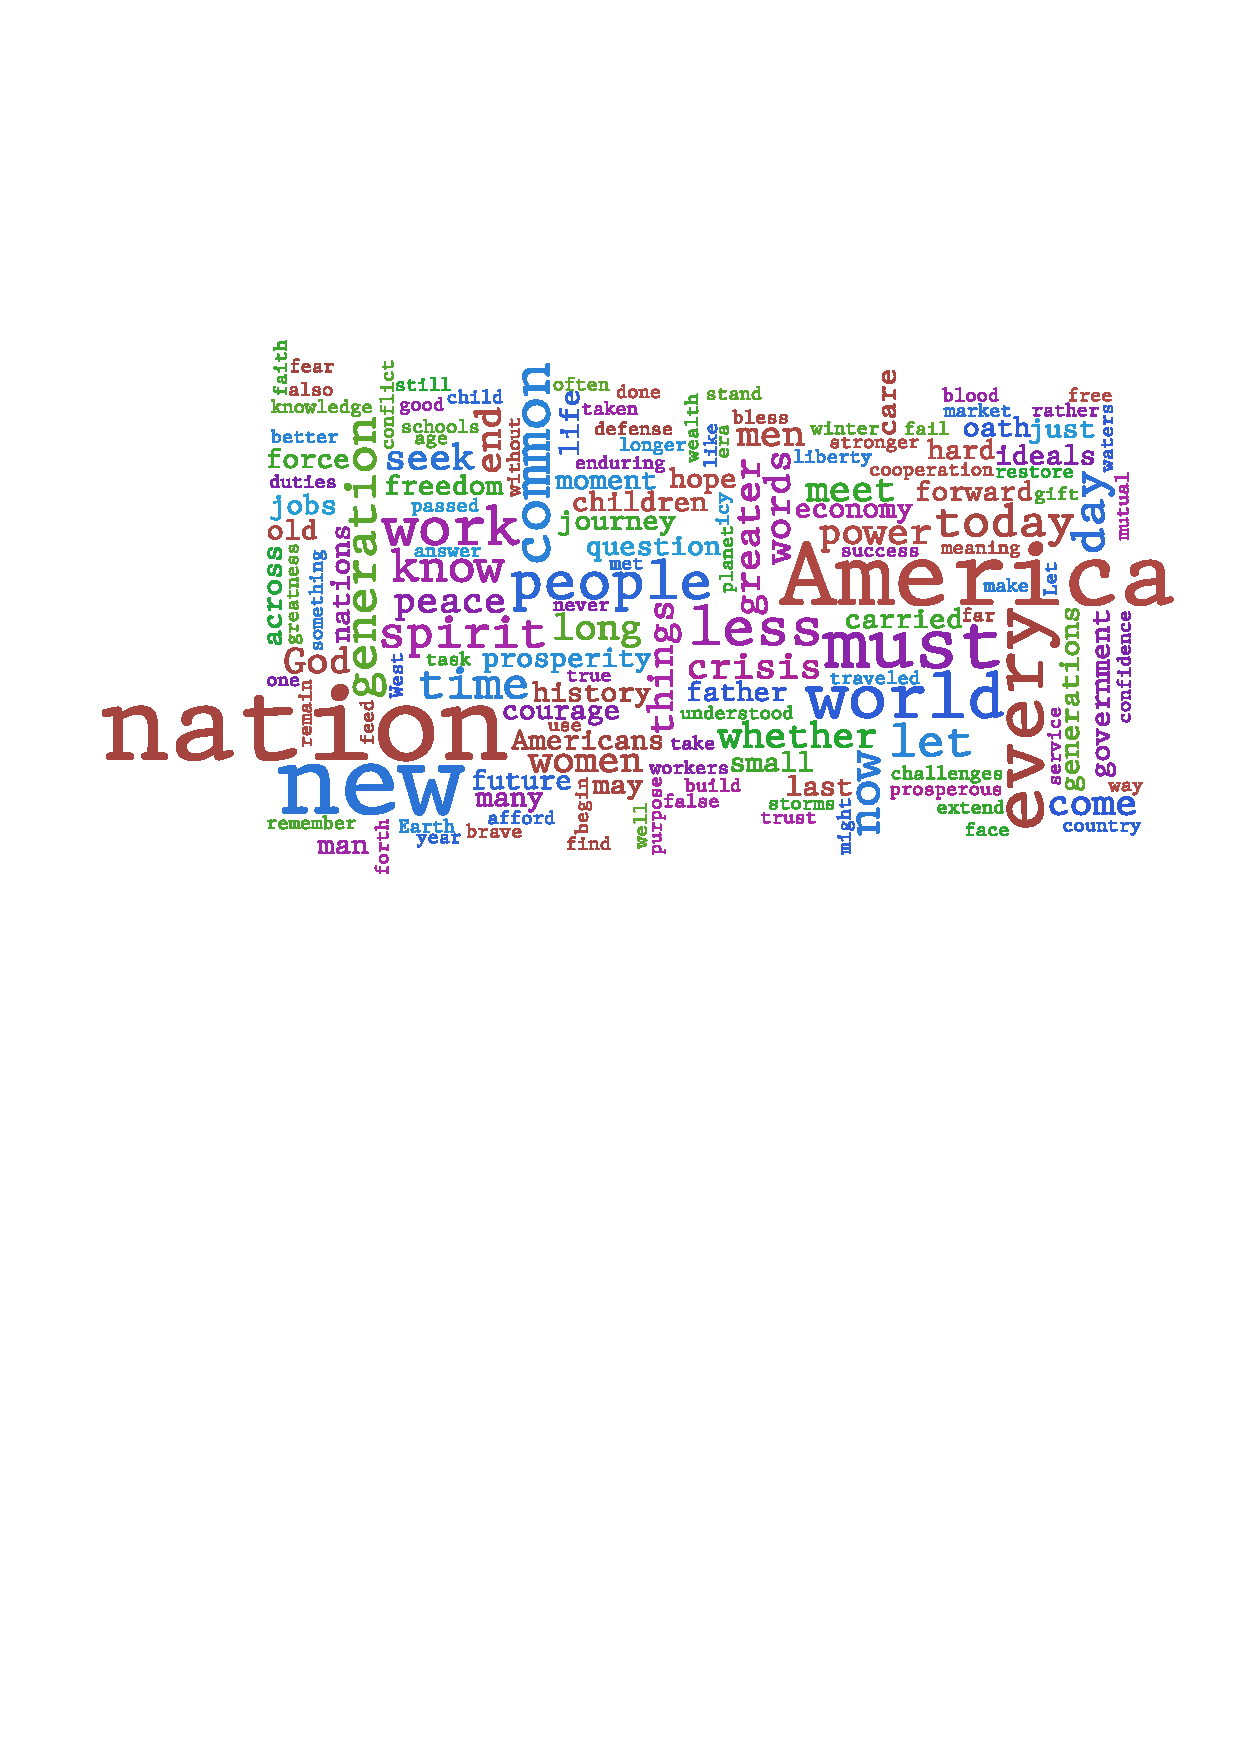
\includegraphics[width=10cm]{obamawordle.pdf}
 \end{center}
\end{frame}




\begin{frame}
 \frametitle{Sample v. ``population''}
 \begin{itemize}
  \item Basic Idea: Observed text is a stochastic realization
  \item Systematic features shape most of observed verbal content
  \item Non-systematic, random features also shape verbal content
 \end{itemize}
 \begin{center}
  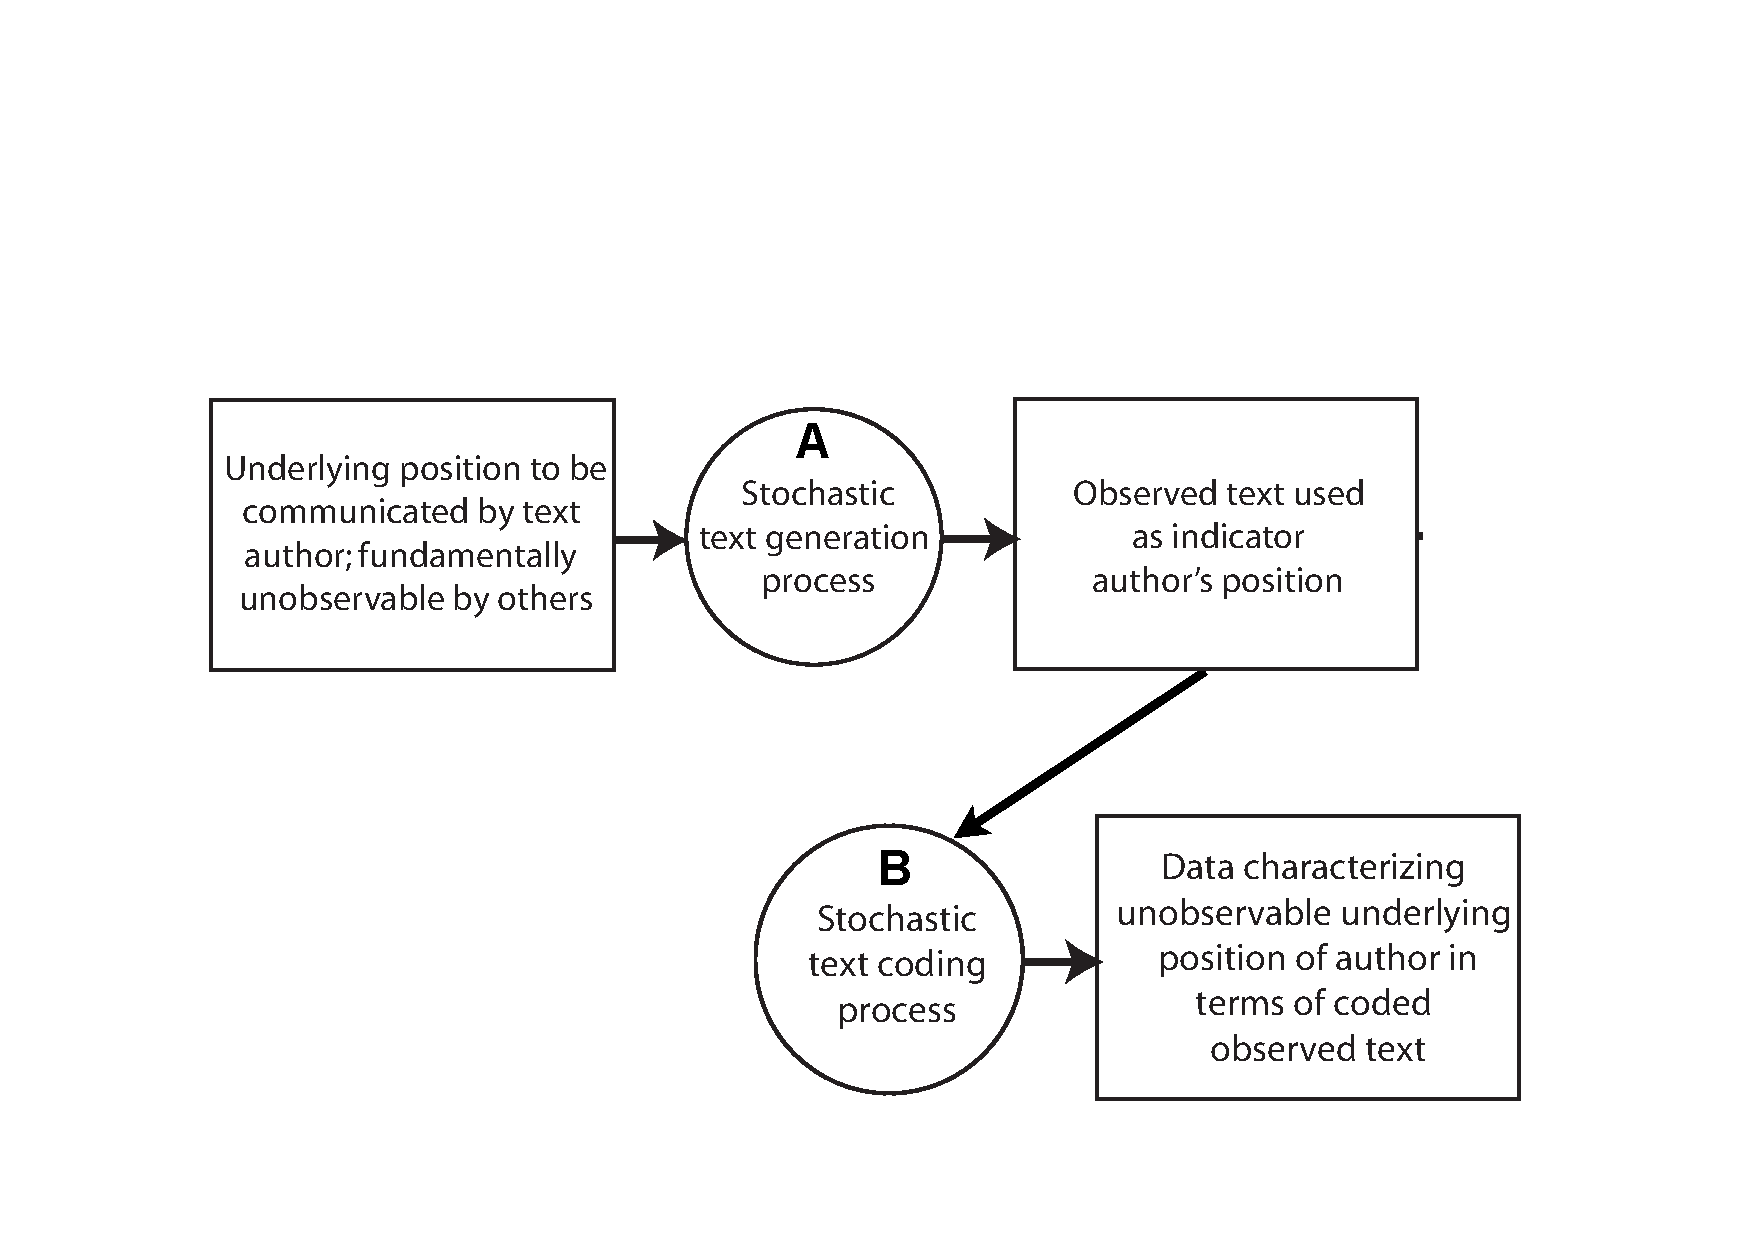
\includegraphics[width=8cm]{process2.pdf}
 \end{center}
\end{frame}


\begin{frame}
 \frametitle{Implications of a stochastic view of text}
 \begin{itemize}
  \item Observed text is not the only text that could have been generated
  \item Very different if you are trying to monitor something like
        hate speech, where what you actually say matters, not the value of
        your ``expected statement''
  \item Means that having ``all the text'' is still not a ``population''
  \item Suggests you could employ bootstrapping strategies to estimate
        uncertainty for sample statistics, even things like readability
 \end{itemize}
\end{frame}





\section{Bootstrapping}

\begin{frame}
 \frametitle{Bootstrapping}
 \begin{itemize}
  \item \emph{Bootstrapping} refers to repeated resampling of data
        points \alert{with replacement}
  \item Used to estimate the error variance (i.e.\@ the \alert{standard
   error}) of an estimate when the sampling distribution is unknown
   (or cannot be safely assumed)
   \item Robust in the absence of parametric assumptions
   \item Useful for some quantities for which there is no known
         sampling distribution, such as computing the standard error of a median
  \end{itemize}
 \end{frame}

 \begin{frame}[fragile]
  \frametitle{Bootstrapping illustrated}
  \footnotesize
  \begin{verbatim}
> ## illustrate bootstrap sampling
> set.seed(30092014)   # set the seed so that your results will match mine!
> # using sample to generate a permutation of the sequence 1:10
> sample(10)
 [1]  4  2  1  9  8  5  7  3  6 10
> # bootstrap sample from the same sequence
> sample(10, replace=T)
 [1] 8 6 6 2 5 8 4 8 4 9
> # boostrap sample from the same sequence with probabilities that
> # favor the numbers 1-5
> prob1 <- c(rep(.15, 5), rep(.05, 5))
> prob1
 [1] 0.15 0.15 0.15 0.15 0.15 0.05 0.05 0.05 0.05 0.05
> sample(10, replace=T, prob=prob1)
 [1] 4 1 1 2 8 3 1 6 1 9
  \end{verbatim}
 \end{frame}


 \begin{frame}[fragile]
  \frametitle{Bootstrapping the standard error of the median}
  Using a user-defined function:
  \footnotesize
  \begin{verbatim}
b.median <- function(data, n) {
    resamples <- lapply(1:n, function(i) sample(data, replace=T))
    sapply(resamples, median)
    std.err <- sqrt(var(r.median))
    list(std.err=std.err, resamples=resamples, medians=r.median)
}
summary(b.median(spending, 10))
summary(b.median(spending, 100))
summary(b.median(spending, 400))
median(spending)
  \end{verbatim}
 \end{frame}

 \begin{frame}[fragile]
  \frametitle{Bootstrapping the standard error of the median}
  Using R's \textbf{boot} library:
  {\footnotesize
   \begin{verbatim}
library(boot)
samplemedian <- function(x, d) return(median(x[d]))
quantile(boot(spending, samplemedian, R=10)$t, c(.025, .5, .975))
quantile(boot(spending, samplemedian, R=100)$t, c(.025, .5, .975))
quantile(boot(spending, samplemedian, R=400)$t, c(.025, .5, .975))
   \end{verbatim}}
  \vspace{3ex}
  \small \alert{Note:} There is a good reference on using \texttt{boot()} from
  \newline \small \url{http://www.mayin.org/ajayshah/KB/R/documents/boot.html}
 \end{frame}

 \begin{frame}
  \frametitle{Bootstrapping methods for textual data}
  \begin{itemize}
   \item Question: what is the "sampling distribution" of a text-based
         statistic?  Examples:
         \begin{itemize}
          \item a term's (relative) frequency
          \item lexical diversity
          \item complexity
         \end{itemize}
  \end{itemize}
 \end{frame}


 \begin{frame}
  \centerline{\huge EQUIVALENCE CLASSES}
 \end{frame}


 \begin{frame}
  \frametitle{Bootstrapping text-based statistics}
  \flushright 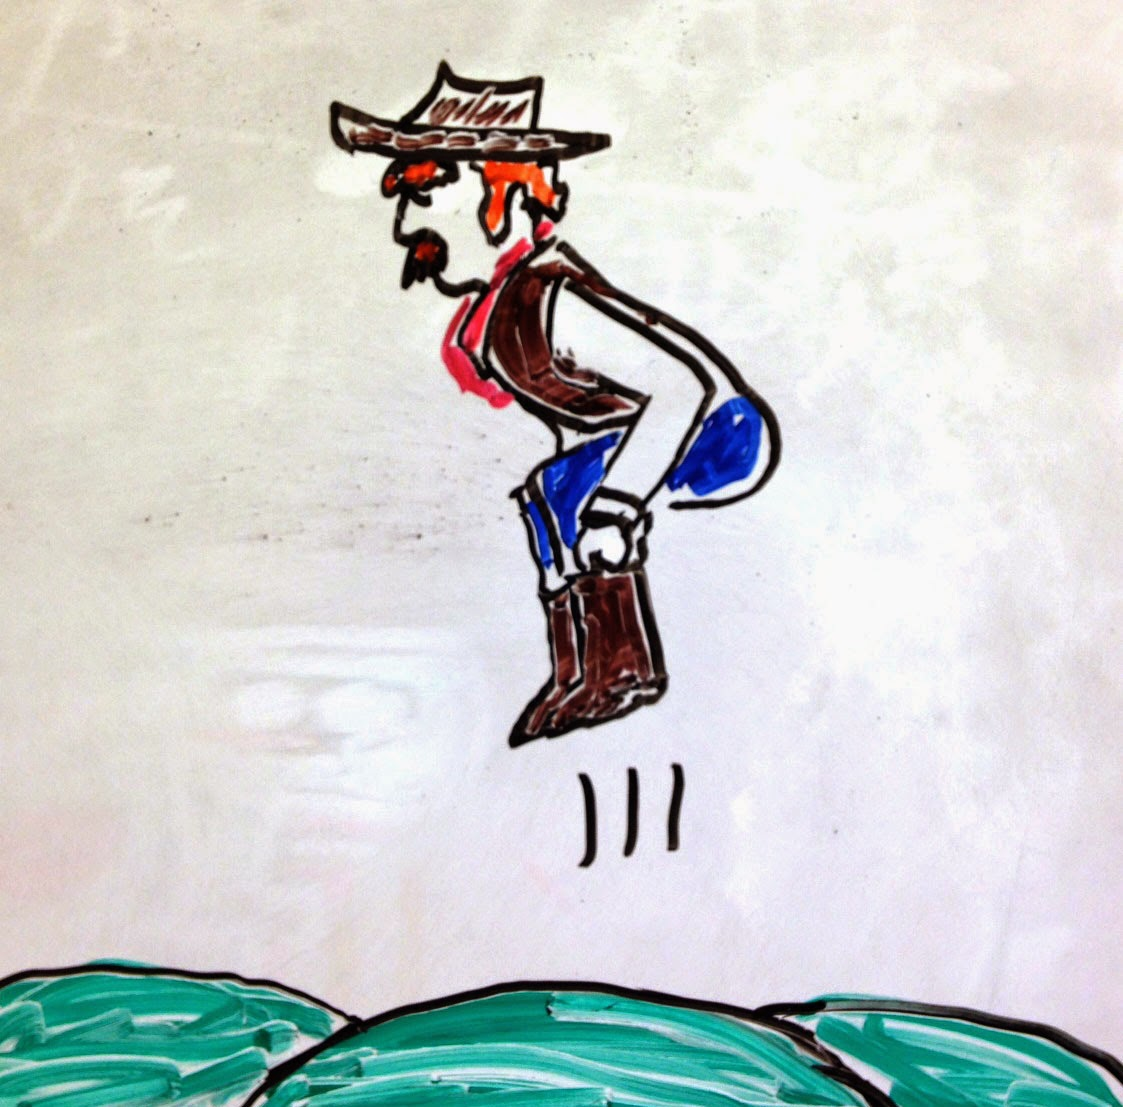
\includegraphics[width=5cm]{bootstraps.png}
 \end{frame}

 \begin{frame}
  \frametitle{Simulation and bootstrapping}

  Used for:
  \begin{itemize}
   \item<1->{Gaining \alert{intuition} about distributions and sampling}
   \item<2->{Providing \alert{distributional} information not
   distributions are not directly known, or cannot be assumed}
   \item<3->{Acquiring \alert{uncertainty} estimates}
  \end{itemize}

  \pause[4] \vspace{2ex} Both simulation and bootstrapping are
  \alert{numerical approximations} of the quantities we are interested
  in. (Run the same code twice, and you get different answers)

  \vspace{2ex}
  Solution for replication: save the \alert{seed}
 \end{frame}
